\documentclass[times,specification,annotation]{style/itmo-student-thesis/itmo-student-thesis}

\usepackage{icomma}
\usepackage{tabularx}
\usepackage{adjustbox}

\usepackage{tikz}
\usetikzlibrary{arrows}

\usepackage{tikz-qtree}
\usepackage{circuitikz}
\usepackage{pdfpages}

\usepackage{filecontents}
\begin{filecontents}{bachelor-thesis.bib}
@article{korneev-elizarov-pcms,
  title={Автоматическое тестирование решений на соревнованиях по программированию},
  author={Корнеев, ГА and Елизаров, РА},
  journal={Телекоммуникации и информатизация образования},
  number={1},
  pages={61--73},
  year={2003}
}
@book{stone1987program,
  title={Program construction},
  author={Stone, Richard Gary and Cooke, Derek John},
  number={22},
  year={1987},
  publisher={Cambridge University Press}
}
@book{mitchell2003concepts,
  title={Concepts in programming languages},
  author={Mitchell, John C and Apt, Krzysztof},
  year={2003},
  publisher={Cambridge University Press}
}
@online{competative-prog-wiki,
    year        = {2023},
    title       = {Competitive programming},
    url         = {https://en.wikipedia.org/w/index.php?title=Competitive_programming&oldid=1145645404},
    year        = {2023},
    langid      = {english}
}
@online{darkcyan-polygon-tutorial,
    year        = {2022},
    title       = {Polygon.Codeforces Tutorial - A Guide to Problem Preparation [Part 1]},
    author      = {Tran Quang Loc},
    url         = {https://quangloc99.github.io/2022/03/08/polygon-codeforces-tutorial.html},
    year        = {2022},
    langid      = {english}
}
@online{codeforces-rules,
    year        = {2012},
    title       = {Правила соревнований Codeforces},
    author      = {Мирзаянов, МР},
    url         = {https://codeforces.com/blog/entry/4088},
    year        = {2012},
    langid      = {russian}
}
@online{nerc-rules,
    year        = {2023},
    title       = {ICPC Northern Eurasia Regional Contest Rules},
    url         = {https://neerc.ifmo.ru/information/contest-rules.html},
    year        = {2023},
    langid      = {english}
}
@online{roi-regionals-requirements,
    year        = {2022},
    title       = {Требования к организации и проведению регионального этапа Всероссийской олимпиады школьников в 2022/2023 учебном году по информатике},
    url         = {https://edsoo.ru/download/1076/?hash=33c893065154553c8704a8a0cbe9860e},
    year        = {2022},
    langid      = {russian}
}
@online{ioi-rules,
    year        = {2022},
    title       = {IOI Competition Rules},
    url         = {https://ioi2022.id/competition-rules/},
    year        = {2022},
    langid      = {english}
}
@online{cf-graders,
    year        = {2019},
    author      = {Мирзаянов, МР},
    title       = {Polygon: расширенные свойства ресурсов (грейдеры)},
    url         = {https://codeforces.com/blog/entry/66916},
    year        = {2019},
    langid      = {english}
}
@article{parr2013definitive,
  title={The definitive ANTLR 4 reference},
  author={Parr, Terence},
  journal={The Definitive ANTLR 4 Reference},
  pages={1--326},
  year={2013},
  publisher={The Pragmatic Bookshelf}
}
@article{aho-compilers,
  title={Компиляторы: принципы, технологии и инструментарий},
  author={Ахо, А and Лам, М and Сети, Рави and Ульман, Дж},
  journal={М.: Вильямс},
  volume={1},
  pages={257},
  year={2008}
}
@book{design-patterns,
  title={Паттерны объектно-ориентированного проектирования},
  author={Эрих, Г. and Ричард, Х. and Роберт, Д. and Джон, В.},
  year={2020},
  publisher={"Издательский дом ""Питер"""}
}
@online{cf-testlib,
    year        = {2015},
    author      = {Мирзаянов, МР},
    title       = {Коротко о testlib.h},
    url         = {https://codeforces.com/testlib},
    year        = {2015},
    langid      = {russian}
}
@book{cppbook,
  title={Язык программирования C++},
  author={Страуструп, Б.},
  year={2011},
  publisher={Бином}
}
@online{cppcin,
    year        = {2021},
    title       = {std::cin, std::wcin},
    url         = {https://en.cppreference.com/w/cpp/io/cin},
    year        = {2021},
    langid      = {english}
}
@online{javascanner,
    year        = {2022},
    title       = {Class Scanner (Java SE 19)},
    url         = {https://download.java.net/java/early_access/panama/docs/api/java.base/java/util/Scanner.html},
    year        = {2022},
    langid      = {english}
}
@book{laurent2001programming,
  title={Programming Web Services with XML-RPC: Creating Web Application Gateways},
  author={Laurent, Simon St and Johnston, Joe and Wilder-James, Edd and Winer, Dave},
  year={2001},
  publisher={" O'Reilly Media, Inc."}
}
@online{protobufdocs,
    year        = {2023},
    title       = {Protocol Buffers},
    url         = {https://protobuf.dev/},
    year        = {2023},
    langid      = {english}
}
@online{pcms2bachelor,
    year        = {2002},
    author      = {Корнеев, ГА},
    title       = {Игровой метод тестирования решений на соревнованиях по программированию и его реализация},
    url         = {https://www.kgeorgiy.info/theses/Korneev_GA_--_Bachelor_thesis.pdf},
    langid      = {russian}
}
@online{ejudgedocs,
    year        = {2023},
    author      = {Чернов, А},
    title       = {Ejudge contest management system},
    url         = {https://ejudge.ru/},
    langid      = {russian}
}
@online{yacontest,
    year        = {2023},
    title       = {Яндекс.Контест},
    url         = {https://contest.yandex.ru/},
    langid      = {russian}
}
@online{codeforces,
    year        = {2023},
    title       = {Codeforces},
    url         = {https://codeforces.com/},
    langid      = {russian}
}
@online{python2docs,
    year        = {2020},
    title       = {Python 2.7.18 documentation},
    url         = {https://docs.python.org/2.7/},
    langid      = {english}
}
@online{python3docs,
    year        = {2023},
    title       = {Python 3.11.3 documentation},
    url         = {https://docs.python.org/3.11/},
    langid      = {english}
}

@online{problem1772F,
    year        = {2022},
    title       = {Задача F. Копия копии копии},
    url         = {https://codeforces.com/contest/1772/problem/F},
    langid      = {russian}
}

\end{filecontents}

\addbibresource{bachelor-thesis.bib}

\begin{document}

\studygroup{M34371}
\title{Автоматизация построения программных компонентов при подготовке задач по спортивному программированию}
\author{Назаров Георгий Дмитриевич}{Назаров Г.Д.}
\supervisor{Корнеев Георгий Александрович}{Корнеев Г.А.}{доцент, к.т.н.}{доцент факультета информационных технологий и программирования}
\publishyear{2023}
\startdate{10}{апреля}{2023}
\finishdate{15}{мая}{2023}

\addconsultant{Мирзаянов М.Р.}{без степени, без звания}

\secretary{Штумпф С.А.}

\technicalspec{
    Требуется разработать систему, автоматизирующую процесс построения программных компонентов при подготовке (разработке) задач по спортивному программированию, в том числе:

    1. Спроектировать специальный язык описания входных и выходных данных, требуемых в задаче по спортивному программированию.

    2. Реализовать систему кодогенерации, которая, на основании описания входных и выходных данных, будет генерировать исходный код программных компонентов задачи, в том числе:

    2.1. Программы, проверяющей ответ участника (чекера);

    2.2. Программы, проверяющей корректность входных данных (валидатора);

    2.3. Компонентов ввода-вывода пользовательских решений задачи (грейдеров).

    3. Внедрить полученную систему в сервис подготовки задач по спортивному программированию «Polygon».
}

\includepdf{include/title.pdf}
\includepdf[pages={1-2}]{include/abstract.pdf}
\includepdf[pages={1-2}]{include/annotation.pdf}

%% Ставим номер страницы сверху по центру
\newcommand{\TheOnlyTruePageStyle}{fancy}
\pagestyle{\TheOnlyTruePageStyle}
\renewcommand{\headrulewidth}{0pt}
\renewcommand{\footrulewidth}{0pt}
\lhead{}
\chead{\thepage}
\rhead{}
\lfoot{}
\cfoot{}
\rfoot{}
\addtolength{\voffset}{3mm}
\addtolength{\headsep}{-3mm}

\setcounter{page}{4}
% Выключаем переносы в оглавлении
\pretocmd{\tableofcontents}{\begingroup\banhyphens}{}{}
\apptocmd{\tableofcontents}{\endgroup}{}{}

\setmonofont{Consolas}

\lstset{
    language=C++,
    extendedchars=\true,
    tabsize=4,
    keywordstyle=\color{darkblue},
    commentstyle=\color{gray},
    stringstyle=\color{darkgreen},
    breaklines=true,
    showstringspaces=false,
    basicstyle=\ttfamily\small,
    showspaces=true
}

\tableofcontents

\startprefacepage

Соревнования по спортивному программированию проходят с использованием автоматизированных систем тестирования~\cite{korneev-elizarov-pcms}, например, PCMS2~\cite{pcms2bachelor}, Ejudge~\cite{ejudgedocs}, Яндекс.Контест~\cite{yacontest}, Codeforces~\cite{codeforces}. Участники отсылают на проверку исходный код программы-решения, которая автоматически проверяется на наборе тестов~\cite{competative-prog-wiki}.

Для того, чтобы задачу по спортивному программированию можно было использовать в автоматизированной тестирующей системе, авторы задачи должны предварительно подготовить <<пакет>> задачи, состоящий из условий задачи, тестов и набора программ, участвующих в процессе тестирования~\cite{darkcyan-polygon-tutorial}. Подготовка каждой задачи~--- трудоемкий ручной процесс, легко подверженный ошибкам.

Целью данной выпускной квалификационной работы является разработка системы, частично автоматизирующей процесс реализации программных компонентов при подготовке задач по спортивному программированию.

В работе спроектирован язык описания входных и выходных данных для задач по спортивному программированию, позволяющий описывать структуру тестов и ожидаемых ответов, а так же указывать ограничения на переменные во входных и выходных данных. Реализована система частичной генерации некоторых программных компонентов задачи. Полученная система внедрена в сервис для подготовки задач по спортивному программированию <<Polygon>>. На работу получен акт о внедрении.

Первая глава работы подробно описывает предметную область~--- описывается процесс подготовки соревнований по спортивному программированию и процесс их проведения. Первая глава содержит описания компонентов задачи, вводятся термины, которые будут использованы в последующих главах.

Во второй главе формулируются и требования к языку описания входных и выходных данных, приводится концептуальное описание спроектированного языка. Вторая глава содержит наглядное описание языковых конструкций на примере задачи с одного из соревнований на платформе Codeforces.

В третьей главе подробно изложены детали реализации разбора языка, более подробно описывается семантика языковых конструкций.

Четвертая глава содержит детали реализации системы генерации исходного кода программных компонентов задачи по описанию входных и выходных данных, описан способ интеграции полученной системы в сервис подготовки задач по спортивному программированию <<Polygon>>, а так же приводится описание процесса тестирования полученной системы.

\chapter{Подготовка и проведение соревнований по спортивному программированию}

В данной главе приводятся описания существующего процесса подготовки задач по спортивному программированию и процесса участия в соревнованиях по спортивному программированию с точки зрения участника. В дальнейшей работе будут использоваться термины и определения, вводимые в этой главе.

\section{Соревнования с точки зрения участников}

На соревнованиях по спортивному программированию участникам предлагается к решению набор задач. За ограниченное количество времени участники должны решить как можно больше задач и как можно точнее (определение <<точности>> зависит от правил конкретного соревнования).

К каждой задаче прилагается условие задачи~--- текстовое человекочитаемое описание требований к решению участника. Решением участника является исходный код на одном из доступных в автоматизированной системе тестирования языков программирования. Решение задачи может содержать, в зависимости от правил соревнования, как весь исходный код программы-решения, так и его часть~--- реализацию заданного в условии задачи интерфейса или функции с необходимой сигнатурой.

После проверки решения, участнику сообщается вердикт проверки~--- строка с информацией о корректности решения, возможно, содержащая дополнительную информацию, например, номер теста, на котором решение участника выдало неправильный ответ~\cite{codeforces-rules},~\cite{nerc-rules}.

\section{Процесс тестирования}

После получения решения участника автоматизированная тестирующая система выполняет его обработку, состоящую из следующих основных шагов~\cite{roi-regionals-requirements}.

\begin{enumerate}[leftmargin=1.75cm]
    \item Компиляция решения участника.
    \item Компоновка (линковка) решения участника с компонентами задачи (при необходимости).
    \item Генерация наборов входных данных (для генерируемых тестов).
    \item Валидация входных данных на соответствие условию задачи.
    \item Запуск исполняемого файла с решением на наборе тестов (входных данных).
    \item Запуск проверяющей программы на каждом из тестов и ответов программы-решения.
\end{enumerate}

В зависимости от правил соревнования шагов может быть больше. Об ошибке на любом из шагов сообщается участнику.

\textit{Тестами (входными данными)} являются файлы с определенной автором задачи структурой. В условии задачи описываются переменные и ограничения на них, а так же описывается порядок их появления во входных данных.

В ответ на каждый тест программа-решение должна сгенерировать файл, называемый \textit{выходными данными}. Выходные данные так же состоят из переменных, описанных в условии задачи.

\section{Подготовка задач}

Чтобы задачу можно было использовать в автоматизированной тестирующей системе, авторы задачи должны подготовить следующие компоненты задачи~\cite{darkcyan-polygon-tutorial}.

\begin{enumerate}[leftmargin=1.75cm]
    \item Условия задачи, возможно, на нескольких языках.
    \item Валидатор (от англ. \textit{validator})~--- программу, принимающую на вход произвольный текстовый файл и выдающую вердикт, может ли быть этот файл использован в качестве теста в конкретной задачи. Валидатор должен проверять структуру файла и соответствие значений переменных ограничениям из условия.
    \item Проверяющую программу (альтернативное название~--- чекер, от англ. \textit{checker}, именно оно будет использоваться далее в тексте)~--- программу, принимающую на вход тест, ответ программы участника и ответ жюри (авторского решения), и выдающая вердикт о корректности ответа участника. Чекер дожен проверять выполнение в ответе ограничений из условия задачи.
    \item Тесты (входные данные)~--- файлы, которые будут подаваться на вход решению участника. Могут быть заданы вручную или генерироваться во время тестирования.
    \item Генераторы~--- программы, принимающие в аргументах командной строки параметры, на основании которых генерируют (выводят) тест или набор тестов.
    \item Решение жюри (авторское решение)~--- исходный код эталонного решения задачи. Используется для получения эталонных ответов при запуске чекера.
\end{enumerate}

На некоторых соревнованиях от участников не требуется полная реализация решения, а только лишь его части~--- функции с заданной сигнатурой или интерфейса. Подобные правила применяются, например, на IOI~--- международной олимпиаде по информатике~\cite{ioi-rules}. В таком случае авторам задачи так же необходимо подготовить грейдеры (от англ. \textit{grader}, <<оценщик>>)~--- часть исходного кода решения, которая будет скомпонована (слинкована) с решением участника. Исходный код грейдеров должен обязательно содержать точку входа программы и реализацию ввода-вывода, специфичную для задачи. Опционально, грейдеры могут выполнять дополнительные действия перед передачей управления коду участника или после окончания исполнения кода участника. Грейдеры должны быть написаны на каждом из доступных участнику языков программирования~\cite{cf-graders}.

\section{Примеры программных компонентов задачи}

Рассмотрим подробнее программные компоненты на примере задачи <<A~+~B>>.

Дано два целых числа: $a$ и $b$. Требуется вывести их сумму.

В единственной строке входных данных задано два целых числа $a$ и $b$ ($-1000 \le a, b \le 1000$), разделенных пробелом.

В единственной строке выходных данных требуется вывести значение $a + b$.

Листинг~\ref{a-plus-b-validator} содержит исходный код валидатора на языке программирования C++~\cite{cppbook} с применением библиотеки \texttt{testlib.h}~\cite{cf-testlib}. В первой строке функции \texttt{main()} вызывается функция инициализации библиотеки \texttt{testlib.h} в режиме валидатора. Затем считывается два целочисленных значения в интервале от $-1000$ до $1000$, разделенных одним пробелом. Затем ожидается перевод строки и конец файла теста. Для считывания данных используется объект \texttt{inf} из библиотеки \texttt{testlib.h}, отвечающий за поток ввода данных.

\begin{lstlisting}[float=!h,caption={Пример валидатора},label={a-plus-b-validator},language=c++]
#include "testlib.h"

int main(int argc, char *argv[])
{
    registerValidation(argc, argv);
    inf.readInt(-1000, 1000, "a");
    inf.readSpace();
    inf.readInt(-1000, 1000, "b");
    inf.readEoln();
    inf.readEof();
    return 0;
}
\end{lstlisting}

Листинг~\ref{a-plus-b-checker} содержит исходный код чекера. В первой строке функции \texttt{main()} вызывается функция инициализации библиотеки \texttt{testlib.h} в режиме чекера. Затем считывается одно целочисленное значение в интервале от $-2000$ до $2000$ два раза: сначала ответ участника, затем ответ жюри (вывод авторского решения). Ответ участника считывается при помощи объекта \texttt{ouf}, ответ жюри~--- при помощи объекта \texttt{ans}. Если ответы совпали, участник получает вердикт <<правильный ответ>>, в противном случае <<неправильный ответ>>, на соответствующем тесте. Для выдачи вердикта используется функция \texttt{quitf()} из библиотеки \texttt{testlib.h}, осуществляющая форматированный вывод вердикта и завершающая исполнение чекера с кодом возврата, соответствующем вердикту. В случае правильного ответа код возврата равен $0$, в случае неправильного~--- $1$.

\begin{lstlisting}[float=!h,caption={Пример чекера},label={a-plus-b-checker},language=c++]
#include "testlib.h"

int readAns(InStream& stream)
{
    return stream.readInt(-2000, 2000, "sum");
}

int main(int argc, char *argv[])
{
    registerTestlibCmd(argc, argv);
    int participant = readAns(ouf);
    int jury = readAns(ans);
    if (participant != jury)
        quitf(_wa, "Wrong answer");
    else
        quitf(_ok, "Ok");
}
\end{lstlisting}

Тесты могут быть сгенерированы программно. Листинг~\ref{a-plus-b-generator} содержит исходный код генератора случайных тестов, который принимает на вход единственный аргумент командной строки~--- ограничение на абсолютную величину генерируемых значений. В первой строке функции \texttt{main()} вызывается функция инициализации библиотеки \texttt{testlib.h} в режиме генератора. Затем происходит разбор аргументов командной строки при помощи функции \texttt{opt<>()} из библиотеки \texttt{testlib.h}. Затем два случайных значения выводятся в стандартный поток вывода через пробел, затем следует перевод строки. Для генерации случайных значений используется объект \texttt{rnd} из библиотеки \texttt{testlib.h}.

\begin{lstlisting}[float=!h,caption={Пример генератора},label={a-plus-b-generator},language=c++]
#include <iostream>
#include "testlib.h"
 
int main(int argc, char* argv[]) {
    registerGen(argc, argv, 1);
 
    int N = opt<int>(1);
    std::cout << rnd.next(-N, N) << ' ';
    std::cout << rnd.next(-N, N) << std::endl;
    return 0;
}
\end{lstlisting}

Грейдеры являются написанной жюри (автором задачи) частью исходного кода, который будет скомпонован с реализацией участника для получения полного исполняемого файла с решением.

\begin{lstlisting}[float=!h,caption={Пример грейдера для языка C++},label={a-plus-b-grader-cpp},language=c++]
// aplusb.h

int sum_ab(int a, int b);

// grader.cpp

#include <iostream>
#include "aplusb.h"
 
int main() {
    int a, b;
    std::cin >> a >> b;
    std::cout << sum_ab(a, b) << std::endl;
    return 0;
}
\end{lstlisting}

Листинг~\ref{a-plus-b-grader-cpp} содержит исходный код грейдера для языка программирования C++. Грейдеры для C++ обычно состоят из двух файлов: заголовочного и главного. В заголовочном файле определены вспомогательные функции, предоставляемые участнику, а так же сигнатуры функций, которые участник должен реализовать. Главный файл содержит точку входа (функцию \texttt{main()}, с которой будет начато исполнение) и код, считывающий входные данные из стандартного потока ввода и выводящий ответ, полученный вызовом пользовательской реализации, в стандартный поток вывода.

Листинг~\ref{a-plus-b-grader-py} содержит исходный код грейдера для языка программирования Python~\cite{python3docs}. Так как Python~--- интерпретируемый язык программирования, понятие линковки для него не определено, поэтому грейдер напрямую импортирует и вызывает решение участника. Блок кода в середине содержит проверку версии языка, чтобы грейдер мог работать как на Python 2~\cite{python2docs}, так и на Python 3~\cite{python3docs}.

\begin{lstlisting}[caption={Пример грейдера для языка Python},label={a-plus-b-grader-py},language=python]
import solution
import sys

if sys.version_info[0] < 3:
    _input = raw_input
else:
    _input = input
 
a, b = map(int, _input().split())
print(solution.sum_ab(a, b))
\end{lstlisting}

\section{Цели и задачи ВКР}

В предыдущих пунктах показано, что для подготовки даже простых задач по спортивному программированию авторам задачи необходимо проделать существенную работу, написав исходный код для, как минимум, трёх программных компонентов~--- валидатора, чекера и генератора, при этом генераторов может быть много, для того, чтобы сгенерировать как можно более разнообразные тесты. При этом, в случае, если задача подразумевает наличие грейдеров, объем исходного кода, необходимого к написанию, становится пропорциональным количеству поддерживаемых тестирующей системой языков программирования.

% Задание на ВКР

Основная цель данной выпускной квалификационной работы~--- разработка системы, автоматизирующей процесс реализации программных компонентов при подготовке задач по спортивному программированию.

В результате анализа существующего процесса подготовки задач соревнований были выделены следующие задачи, решаемые в данной выпускной квалификационной работе.

\begin{enumerate}[leftmargin=1.75cm]
    \item Необходимо спроектировать специальный язык описания входных и выходных данных, специфичных для задачи.
    \item Реализовать систему кодогенерации, которая будет принимать на вход описание входных и выходных данных, на основании которой будет частично сгенерирован исходный код валидатора, чекера и грейдеров.
    \item Внедрить реализованную систему в сервис подготовки задач по спортивному программированию <<Polygon>>.
\end{enumerate}

\chapterconclusion

В этой главе был описан процесс подготовки и проведения соревнований по спортивному программированию, приведен перечень программных компонентов задач. Было показано, что данная выпускная квалификационная работа актуальна, так как существующий процесс подготовки задач требует от жюри высокого уровня внимательности. В конце главы были сформулированны цели и задачи выпускной квалификационной работы.

\chapter{Проектирование языка описания входных и выходных данных}

В этой главе формулируются требования к языку описания входных и выходных данных и описывается разработанный язык описания входных и выходных данных.

\section{Требования к языку описания}

Были выделены следующие требования к возможностям языка описания.

\begin{enumerate}[leftmargin=1.75cm]
    \item Должна быть возможность указывать название для каждой переменной. Это необходимо для генерации человекочитаемых сообщений об ошибках в валидаторе и чекере.
    \item Должна быть возможность указывать тип переменных, для корректной реализации ввода-вывода.
    \item Должна быть возможность описывать структуры~--- упорядоченный набор семантически связных переменных.
    \item Должна быть возможность указывать места перевода строк.
    \item Должна быть возможность задавать ограничения на переменные~--- для проверки корректности данных.
\end{enumerate}

Отдельно стоит отметить одно неформальное требование: язык описания должен иметь <<низкий порог входа>>. Иными словами, <<простые>> входные и выходные данные должны с его помощью описываться <<простыми>> конструкциями.

Так же для удобства последующей реализации было принято решение ограничить возможный язык описания классом $LL(1)$.

\section{Концептуальное описание языка}\label{lang-concepts}

Входные и выходные данных представляют собой текстовые файлы, содержимое которых удовлетворяет описанным в условии задачи ограничениям и формату. Разработанный язык описания представляет способ текстового машиночитаемого описания структуры входных и выходных данных, понятного человеку. 

В этом разделе мы рассмотрим лексику и синтаксис языка описания входных и выходных данных на примере задачи <<Копия копии копии>> с соревнования <<Codeforces Round 839 (Div. 3)>>~\cite{problem1772F}. С условием задачи можно ознакомиться в Приложении~\ref{statement1772F}. Листинг~\ref{iomarkupfullexample} содержит описание входных и выходных данных для этой задачи.

\begin{lstlisting}[
    float=!h,
    caption={Пример описания ввода-вывода},
    keywordstyle=\color{black},
    commentstyle=\color{black},
    stringstyle=\color{black},
    label={iomarkupfullexample}
]
# https://codeforces.com/contest/1772/problem/F

picture (n: int32, m: int32) {
    s: string[i=1..n, sep='\n'] | len(s[i]) == m;
}

input {
    n: int32 | 3 <= n && n <= 30;
    m: int32 | 3 <= m && m <= 30;
    k: int32 | 0 <= k && k <= 100;
    eoln;
    eoln;

    pictures: picture(n, m)[i=1..k + 1, sep="\n\n"];
}

output {
    startPicIndex: int32 | 1 <= startPicIndex
                           && startPicIndex <= input.k + 1;
    eoln;
    q: int32 | 0 <= q && q <= 10 ** 7;
    eoln;
    ops: array[j=1..q, sep='\n'] of {
        op: int32;
        if (op == 1) {
            x: int32 | 2 <= x && x <= input.n - 1;
            y: int32 | 2 <= y && y <= input.m - 1;
        } else {
            i: int32 | 1 <= i && i <= input.k + 1;
        }
    };
}

\end{lstlisting}

Файл описания входных и выходных данных состоит из набора \textit{структур}~--- объявлений семантически объединенных переменных, идущих во входных или выходных данных в указанном в описании порядке. Структуры можно рассматривать как функции, тело которых состоит из описания того, какие переменные нужно считывать или выводить и где ожидаются переводы строк. В примере можно видеть три структуры: \texttt{picture}, \texttt{input} и \texttt{output}. При этом, наличие структур \texttt{input} и \texttt{output} обязательно, так как они описывают непосредственно входные и выходные данные. Переменные внутри структуры могут представлять собой значения, массивы или другие структуры.

Любая структура, за исключением \texttt{input} и \texttt{output} может иметь \textit{параметры}, семантически похожие на аргументы функции. В примере у структуры \texttt{picture} есть два параметра: \texttt{n} и \texttt{m}.

Структуры могут содержать переменные, условные операторы и модификаторы ввода-вывода. В примере структура \texttt{input} содержит четыре переменные: \texttt{n}, \texttt{m}, \texttt{k} и \texttt{pictures}.

Модификаторы ввода-вывода используются для изменения разделителей между переменными и указания необходимого форматирования во входных и выходных данных. В примере в структуре \texttt{input} есть два вхождения модификатора \texttt{eoln}. Такая запись означает, что переменные \texttt{n}, \texttt{m} и \texttt{k} находятся на одной строке во вводе, затем следует два перевода строки и затем переменная \texttt{pictures}. На данный момент поддерживается только модификатор \texttt{eoln}, означающий перевод строки.

Условные операторы используются для изменения набора переменных в структуре в зависимости от какого-либо условия. В примере в структуре \texttt{output} содержится условный оператор. Листинг~\ref{iomarkupifexample} содержит пример условного оператора. Когда считывание входных данных или вывод выходных данных доходит до условного оператора, вычисляется условие, в данном случае \texttt{op == 1}. Если оно истино, далее будут считаны (или выведены) переменные из первого (положительного) блока, в данном случае \texttt{x} и \texttt{y}. Если же условие ложно, то будут считаны переменные из второго (отрицательного) блока, в данном случае \texttt{i}.

\begin{lstlisting}[
    float=!h,
    caption={Пример условного оператора},
    keywordstyle=\color{black},
    commentstyle=\color{black},
    stringstyle=\color{black},
    label={iomarkupifexample}
]
if (op == 1) {
    x: int32 | 2 <= x && x <= input.n - 1;
    y: int32 | 2 <= y && y <= input.m - 1;
} else {
    i: int32 | 1 <= i && i <= input.k + 1;
}
\end{lstlisting}

Объявление переменной содержит название соответствующей переменной, её тип и, возможно, ограничение на эту переменную, представленное логическим выражением. Рассмотрим объявление переменной \texttt{x} из листинга~\ref{iomarkupifexample}. Сначала записано <<\texttt{x}>>~--- название переменной, затем следует <<\texttt{int32}>>~--- её тип, и после следует <<\texttt{2 <= x \&\& x <= input.n - 1}>>~--- ограничение на переменную.

Для построения лексического и синтаксического анализаторов языка описания был использован генератор нисходящих анализаторов для формальных языков ANTLR~4~\cite{parr2013definitive}. Приложение~\ref{appendix-antlr-grammar} содержит полное описание грамматики языка в формате ANTLR~4. Листинг~\ref{appendix-lexer-src} содержит определения типов токенов, листинг~\ref{appendix-grammar-src} содержит грамматику языка описания ввода-вывода, листинг~\ref{appendix-grammar-pl-src} содержит грамматику подъязыка для записи выражений. Далее в этой главе будут рассматриваться различные поддерживаемые языковые конструкции, поэтому, в тексте этой главы выражения <<тип токена \texttt{X}>> и <<нетерминал \texttt{X}>> следует рассматривать как ссылки на соответствующие определения из приложения~\ref{appendix-antlr-grammar}.

Типы токенов \texttt{LINE\_COMMENT}, \texttt{COMMENT} и \texttt{WS} отвечают за комментарии и пробельные символы. Такие токены должны впоследствии игнорироваться синтаксическим анализатором, что указано директивой \texttt{-> skip} после них. Однострочные комментарии начинаются с символа <<\texttt{\#}>> и продолжаются до конца строки. Блоковые комментарии обрамляются последовательностями символов <<\texttt{/*}>> и <<\texttt{*/}>>. Листинг~\ref{iomarkupcommentsexample} содержит примеры комментариев.

\begin{lstlisting}[
    float=!h,
    caption={Примеры комментариев},
    keywordstyle=\color{black},
    commentstyle=\color{black},
    stringstyle=\color{black},
    label={iomarkupcommentsexample}
]
# Пример однострочного комментария (LINE_COMMENT)

/*
    Пример
    многострочного
    комментария
    (COMMENT)
*/
\end{lstlisting}

Тип токена \texttt{NAME} отвечает за идентификаторы. Листинг~\ref{iomarkupifexample} содержит примеры идентификаторов: <<\texttt{op}>>, <<\texttt{x}>>, <<\texttt{y}>>, <<\texttt{n}>>, <<\texttt{m}>>, <<\texttt{k}>> и <<\texttt{input}>>. Для упрощения последующей кодогенерации, идентификаторы могут содержать только буквы английского алфавита, и символы <<\texttt{\_}>>, <<\texttt{0}>>~-- <<\texttt{9}>>.

\section{Подъязык выражений}\label{syntax-pl-section}

В языке описания входных и выходных данных можно выделить подъязык для записи выражений. Выражения можно использовать при записи ограничений на переменные, как показано в листинге~\ref{iomarkupifexample}, или при указании длин массивов. Листинг~\ref{iomarkupexpressionsexample} содержит примеры выражений. Список всех поддерживаемых в выражениях операций содержится в приложении~\ref{appendix-pl-operators-priority} в таблице~\ref{pl-operators-priority}.

Язык записи выражений сделан максимально близким по виду и семантике к языку C++, чтобы облегчить его использование авторам задач, так как большинство задач по спортивному программированию подготавливаются именно на этом языке программирования. Приоритеты операторов так же идентичны таковым из языка программирования C++.

Листинг~\ref{appendix-grammar-pl-src} содержит полную грамматику подъязыка выражений в формате ANTLR 4. Стартовым нетерминалом является \texttt{plExpression}. 

\begin{lstlisting}[
    float=!h,
    caption={Примеры выражений},
    keywordstyle=\color{black},
    commentstyle=\color{black},
    stringstyle=\color{black},
    label={iomarkupexpressionsexample}
]
# Примеры констант
'a' # Одиночный символ - токен CHAR
"abacaba" # Строка - токен STRING
true # Истина - токен TRUE
false # Ложь - токен FALSE
123 # Целое число - токен NUM_VALUE

2 <= x && x <= input.n - 1

0 <= q && q <= 10u ** 7

(op == 1 || op == 2) ? "1 or 2" : "false"
\end{lstlisting}

Типы токенов \texttt{CHAR} и \texttt{STRING} отвечают за символьные и строковые константы соответственно. Одиночные символы обрамляются машинописными апострофами (<<\texttt{'}>>), строки обрамляются машинописными кавычками (<<\texttt{"}>>).

Типы токенов \texttt{TRUE}~(<<\texttt{true}>>) и \texttt{FALSE}~(<<\texttt{false}>>) отвечают за логические константы <<истина>> и <<ложь>> соответственно.

Токены типа \texttt{NUM\_VALUE} могут содержать целочисленные значения или числа с плавающей точкой (в том числе в экспоненциальной форме записи). Используя суффиксы можно явно указать тип, в который будет транслироваться токен при кодогенерации.

\begin{enumerate}[leftmargin=1.75cm]
    \item Целое значение без суффикса (например, <<\texttt{25}>>) будет иметь тип \texttt{int32}.
    \item Целое значение с суффиксом <<\texttt{U}>> или <<\texttt{u}>>~(например, <<\texttt{10u}>>) будет иметь тип \texttt{uint32}.
    \item Целое значение с суффиксом <<\texttt{L}>> или <<\texttt{l}>>~(например, <<\texttt{123L}>>) будет иметь тип \texttt{int64}.
    \item Целое значение с суффиксом <<\texttt{UL}>> или <<\texttt{ul}>>~(например, <<\texttt{1234ul}>>) будет иметь тип \texttt{uint64}.
\end{enumerate}

Значение считается числом с плавающей точкой, если оно содержит точку, экспоненту или суффикс <<\texttt{f}>>. Примерами записи чисел с правающей точкой являются, <<\texttt{1.0}>>, <<\texttt{1e9}>>, <<\texttt{2f}>> и <<\texttt{1e2f}>>. При наличии суффикса <<\texttt{f}>> считается, что значение имеет тип \texttt{float32}, иначе~--- \texttt{float64}.

Нетерминал \texttt{plValue} отвечает за запись константных значений, он раскрывается в один из токенов, описанных выше.

Типы токенов \texttt{LOGICAL\_AND}~(<<\texttt{\&\&}>>), \texttt{LOGICAL\_OR}~(<<\texttt{||}>>) и \texttt{LOGICAL\_NOT}~(<<\texttt{!}>>) отвечают за операторы логической конъюнкции, дизъюнкции и отрицания. 

За операции <<Побитовое И>>, <<Побитовое исключающее ИЛИ>>, <<Побитовое ИЛИ>> и <<Побитовое отрицание>> отвечают типы токенов \texttt{BITWISE\_AND}~(<<\texttt{\&}>>), \texttt{BITWISE\_XOR}~(<<\texttt{\textasciicircum}>>), \texttt{PIPE}~(<<\texttt{|}>>) и \texttt{BITWISE\_NOT}~(<<\texttt{\textasciitilde}>>) соответственно.

Типы токенов \texttt{EQUALS}~(<<\texttt{==}>>), \texttt{NOT\_EQUALS}~(<<\texttt{!=}>>), \texttt{LESS\_EQUAL}~(<<\texttt{<=}>>), \texttt{GREATER\_EQUAL}~(<<\texttt{>=}>>), \texttt{LESS}~(<<\texttt{<}>>) и \texttt{GREATER}~(<<\texttt{>}>>) отвечают за операторы сравнения: равенство, неравенство, <<меньше или равно>>, <<больше или равно>>, <<меньше>> и <<больше>> соответственно.

Далее следует блок типов токенов, отвечающих за арифметические операции: \texttt{PLUS}~(<<\texttt{+}>>), \texttt{MINUS}~(<<\texttt{-}>>), \texttt{POW}~(<<\texttt{**}>>), \texttt{MULTIPLICATION}~(<<\texttt{*}>>), \texttt{DIVISION}~(<<\texttt{/}>>), \texttt{MODULO}~(<<\texttt{\%}>>)~--- сложение, вычитание, возведение в степень, умножение, деление и взятие остатка от деления соответственно. 

Последняя строка листинга~\ref{iomarkupexpressionsexample} содержит пример использования тернарного оператора, к которому относятся типы токенов \texttt{QUESTION}~(<<\texttt{?}>>) и \texttt{COLON}~(<<\texttt{:}>>).

Нетерминал \texttt{plVarBinding}, раскрывающийся в токен типа \texttt{NAME}, отвечает за переменные в выражениях. Операторы языка выражений и остальные нетерминалы представлены в таблице~\ref{pl-operators-priority}. Стартовым нетерминалом грамматики подъязыка выражений является \texttt{plExpression}. Так же в выражениях можно использовать круглые скобки для изменения приоритета выполнения операций, вызовы встроенных функций (например, функции \texttt{len()} для массивов).

\section{Языковые конструкции}

Рассмотрим языковые конструкции языка описания ввода-вывода.

Определение каждой структуры начинается с токена с типом \texttt{NAME}~--- названия соответствующей структуры. Названия структур должны быть уникальными и не совпадать с названиями встроенных типов. Затем следует необязательные параметры структуры (нетерминал \texttt{namedStructParameters}) и после них описание структуры (нетерминал \texttt{struct}).

Параметры структуры состоят из списка объявлений параметров (нетерминалы \texttt{parameterDeclaration}), разделенных запятыми, обрамленного круглыми скобками (типы токенов \texttt{LPAR} и \texttt{RPAR}). Каждое объявление параметра состоит из имени параметра (\texttt{NAME}) и названия типа этого параметра, разделенных символом двоеточия.

Листинг~\ref{iomarkupstructexample} содержит пример объявления структуры. В примере <<\texttt{picture}>> является названием структуры, <<\texttt{(n: int32, m: int32)}>>~--- списком параметров структуры. Тело структуры находится между открывающей и закрывающей фигурными скобками (типы токенов \texttt{LBRACE} и \texttt{RBRACE}).

\begin{lstlisting}[
    float=!h,
    caption={Пример простой структуры},
    keywordstyle=\color{black},
    commentstyle=\color{black},
    stringstyle=\color{black},
    label={iomarkupstructexample}
]
picture (n: int32, m: int32) {
    s: string[i=1..n, sep='\n'] | len(s[i]) == m;
}
\end{lstlisting}

Тело структуры состоит из списка элементов описания (нетерминалы \texttt{structItem}), обрамленного фигурными скобками. Элементами описания могут быть условные операторы (нетерминал \texttt{conditionalAlternative}), объявления переменных (нетерминал \texttt{variableDeclaration}) или модификаторы ввода-вывода (нетерминал \texttt{ioModifier}). Листинг~\ref{iomarkupstructitemsexample} содержит пример структуры, содержащий все возможные элементы. Строки <<\texttt{startPicIndex: int32;}>>, <<\texttt{q: int32;}>> и другие подобные являются объявлениями переменных, строки <<\texttt{eoln;}>>~--- модификаторами ввода-вывода. Так же на примере показано использование условного оператора <<\texttt{if (...) \{...\} else \{...\}}>>.

\begin{lstlisting}[
    float=!h,
    caption={Пример сложной структуры},
    keywordstyle=\color{black},
    commentstyle=\color{black},
    stringstyle=\color{black},
    label={iomarkupstructitemsexample}
]
output {
    startPicIndex: int32;
    eoln;
    q: int32;
    eoln;
    ops: array[j=1..q, sep='\n'] of {
        op: int32;
        if (op == 1) {
            x: int32;
            y: int32;
        } else {
            i: int32;
        }
    };
}

\end{lstlisting}

Объявления переменных состоят из названия переменной, затем следует символ двоеточия (токен \texttt{COLON}), после него пишется тип переменной (нетерминал \texttt{variableType}). Затем, опционально, следует символ вертикальной черты (тип токена \texttt{PIPE}) и выражение, содержащее ограничение на переменную. Завершается описание переменной символом точки с запятой (тип токена \texttt{SEMICOLON}).

Тип переменной задается следующим образом. Сначала записывается название типа (предопределенное или название объявленной автором задачи структуры), затем, опционально, следуют параметры структуры (нетерминал \texttt{namedTypeParameters}), состоящие из списка выражений, после чего, опционально, следуют одно или несколько деклараций массива (нетерминалы \texttt{arrayParameters}).

Листинг~\ref{iomarkupvarssexample} содержит примеры записи типов для переменных. Первый пример~--- объявление переменной встроенного типа \texttt{int32}. Второй пример~--- объявление переменной, содержащей структуру. Можно заметить, что первый и второй примеры отличаются только названием типа.

Третий пример показывает объявление переменной, содержащей структуру с параметрами. Здесь <<\texttt{picture}>>~--- название структуры, <<\texttt{n * 2}>> и <<\texttt{m + 1}>>~--- выражения аргументов, значения которых будут переданы в структуру.

Рассмотрим четвертый и пятый примеры, в которых объявляются массивы. Чтобы объявить массив, после типа элементов массива записываются \textit{параметры массива}. Параметры массива состоят из объявления переменной итерирования с указанием начального и конечного значений итерирования (нетерминал \texttt{arrayIterationRange}). Затем, через запятую, указывается разделитель переменных в массиве~--- строка, состоящая из пробелов или экранированных переводов строк (нетерминал \texttt{sepValue}).

В примерах переменная итерирования~--- <<\texttt{i}>>. В четвертом примере индексы массива пробегают значения от $1$ до $k + 1$ и между соседними элементами массива ожидается два перевода строки. В пятом примере индексы массива пробегают значения от $1$ до $n$ и между соседними элементами массива ожидается символ пробела.

\begin{lstlisting}[
    float=!h,
    caption={Примеры записи типов переменных},
    keywordstyle=\color{black},
    commentstyle=\color{black},
    stringstyle=\color{black},
    label={iomarkupvarssexample}
]
q: int32; # Переменная типа int32

x: somestruct; # Структура без параметров

pic: picture(n * 2, m + 1); # Структура с параметрами

pictures: picture(n, m)[i=1..k + 1, sep="\n\n"]; # Массив структур с параметрами

s: string[i=1..n, sep=' ']; # Массив строк
\end{lstlisting}

Поддержана возможность определения массивов неименованных структур. Примером такого массива является переменная <<\texttt{ops}>> из листинга~\ref{iomarkupstructitemsexample}. Чтобы объявить массив неименованной структуры, в качестве типа переменной указывается конструкция <<\texttt{array ... of}>> (нетерминал \texttt{arrayOfUnnamedStruct}), после которой следует описание структуры. Вместо троеточия пишутся декларации массива.

% Затем следует блок типов токенов, являющихся зарезервированными словами языка описания входных и выходных данных. Это \texttt{SEP}, \texttt{EOLN\_MODIFIER}, \texttt{IF}, \texttt{ARRAY}, \texttt{OF} и \texttt{else}. Типы \texttt{IF} и \texttt{else} используются в условном операторе. Типы \texttt{SEP} и \texttt{EOLN\_MODIFIER} используются при указании разделителя между переменными во входных и выходных данных. Типы \texttt{ARRAY} и \texttt{OF} используются при объявлении массивов неименованных структур.

% todo to


% \subsection{Синтаксис языка описания}\label{syntax-section}

% Листинг~\ref{appendix-grammar-src} содержит формальную грамматику языка описания входных и выходных данных в формате ANTLR. Стартовым символом % грамматики является нетерминал \texttt{ioMarkup}, раскрывающийся в список нетерминалов \texttt{namedStruct}~--- список определений структур.

\section{Система типов}\label{type-system}

Язык описания входных и выходных данных имеет встроенные целочисленные, строковые, символьные, логические типы и тип вещественных чисел с плавающей точкой. Полный список встроенных типов приведен в таблице~\ref{predefined-types}.

\begin{table}[!h]
\caption{Встроенные типы данных}\label{predefined-types}
\centering
\begin{tabular}{|*{3}{c|}}\hline
Тип & Описание & Пример\\\hline
\texttt{bool} & Логический тип & \texttt{true} \\\hline
\texttt{char} & Символьный тип & \texttt{'x'}\\\hline
\texttt{int32} & $32$-х битный целочисленный знаковый тип & \texttt{123} \\\hline
\texttt{uint32} & $32$-х битный целочисленный беззнаковый тип & \texttt{123u} \\\hline
\texttt{int64} & $64$-х битный целочисленный знаковый тип & \texttt{123l} \\\hline
\texttt{uint64} & $64$-х битный целочисленный беззнаковый тип & \texttt{123ul} \\\hline
\texttt{float32} & $32$-х битный тип чисел с плавающей точкой & \texttt{12.3f} \\\hline
\texttt{float64} & $64$-х битный тип чисел с плавающей точкой & \texttt{12.3} \\\hline
\texttt{string} & Строковый тип (массив символов) & \texttt{"abc"} \\\hline
\end{tabular}
\end{table}

Также поддерживаются объявленные пользователем составные типы (структуры), состоящие из упорядоченного набора переменных других, возможно составных, типов.

К любому типу переменной при объявлении может быть дописан суффикс, являющийся декларацией массива. Такая конструкция объявляет массив указанного типа.

Язык описания ввода-вывода имеет статическую типизацию, то есть типы переменных задаются до этапа исполнения и не могут меняться. При этом, в выражениях допускается приведение типов для чисел, следующее правилам из языка C++~--- от меньшего типа к большему.

\chapterconclusion

В этой главе были сформулированы требования к языку описания входных и выходных данных для задач по спортивному программированию. Было приведено концептуальное описание спроектированного языка, описаны языковые конструкции.

\chapter{Разбор и семантика языка описания входных и выходных данных}

В этой главе описываются алгоритмы обработки языка описания входных и выходных данных, а так же реализация соответствующих алгоритмов.

\section{Обработка языка описания}

Был реализован инструмент, принимающий на вход описание входных и выходных данных на описанном выше языке. Обработка происходит в несколько этапов.

\begin{enumerate}[leftmargin=1.75cm]
    \item Лексический разбор.
    \item Синтаксический разбор.
    \item Поиск определений структур.
    \item Разрешение имен и типов, получение абстрактных синтаксических деревьев выражений и структур.
    \item Генерация кода.
\end{enumerate}

Лексический разбор~--- процесс перевода текстового файла, поданного на вход, в список токенов. Синтаксический разбор~--- процесс перевода списка токенов в дерево разбора. Во время синтаксического разбора так же происходит проверка синтаксической корректности последовательности токенов. Эти два этапа выполняются при помощи сгенерированного ANTLR анализатора~\cite{parr2013definitive}.

На следующем этапе выполняется поиск и регистрация имен структур данных, определенных пользователем. Это необходимо для того, чтобы впоследствии, при получении абстрактных синтаксических деревьев структур, знать полный набор именованных типов, существующих в описании. Этот этап выполняется частичным обходом дерева разбора.

Затем выполняется основной этап обработки, включающий в себя получение внутреннего представления, пригодного для последующей генерации кода. Внутреннее представления является набором абстрактных синтаксических деревьев для выражений и структур с дополнительной информацией в вершинах. Так же на этом этапе происходит разрешение имен переменных и типов. Этот этап выполняется обходом дерева разбора. Во время обхода проверяется семантическая корректность, существование используемых типов (в том числе структур), существование переменных, ссылки на которых используются. Во время обхода поддерживается информация о текущей области видимости переменных. Для упрощения реализации, выражения (длины массивов и ограничения) обходятся отдельно.

Последним этапом является непосредственно генерация целевого кода чекера, валидатора и грейдеров. Для каждого генерируемого программного компонента задачи поочередно выполняется генерация определений структур, объявленных автором в файле описания входных и выходных данных, генерация кода ввода и вывода.

\section{Области видимости}

После выполнения лексического и синтаксического разборов, получается абстрактное синтаксическое дерево, содержащее описание ввода-вывода в иерархическом виде. Для дальнейшей работы необходимо знать полный список имен типов, доступных для использования. Помимо стандартных типов это так же могут быть названия пользовательских структур. Полный список известных имен типов необходим для проверки описания ввода-вывода на корректность перед генерацией кода.

Как и в языках программирования~\cite{aho-compilers}, в языке разметки входных и выходных данных предусмотрены области видимости, в том числе вложенные. Каждая пользовательская структура является отдельной областью видимости.

Чтобы значение переменной можно было использовать внутри другой структуры, её необходимо передать в качестве параметра. Листинг~\ref{iomarkupargssexample} содержит пример такой передачи.

\begin{lstlisting}[
    float=!h,
    caption={Пример передачи аргумента},
    keywordstyle=\color{black},
    commentstyle=\color{black},
    stringstyle=\color{black},
    label={iomarkupargssexample}
]
pair(m: int32) {
    x: int32 | x <= m;
    y: int32 | y <= m;
}

input {
    n: int32;
    m: int32;
    eoln;
    p: pair(m);
}

\end{lstlisting}

Реализация областей видимости представленна в решении классом \texttt{Scope}. Он поддерживает информацию о всех именованных сущностях, которые могут быть использованы. Всего их четыре.

\begin{enumerate}[leftmargin=1.75cm]
    \item Именованные типы~--- встроенные типы данных языка описания ввода-вывода и объявленные пользователем структуры.
    \item Конструкторы~--- объекты, связанные со структурами и инкапсулирующие в себе информацию о полях, параметрах структуры и модификаторах ввода-вывода в структуре.
    \item Переменные~--- поля структур.
    \item Функции~--- доступные для вызова встроенные функции (на данный момент присутствует только функция взятия длины массива или строки).
\end{enumerate}

Существует корневая область видимости, содержащая встроенные типы и функции, а так же ссылки на объявленные пользователем структуры и их конструкторы. Каждая область видимости, кроме корневой, содержит ссылку на родительскую. Таким образом, для каждой области видимости по цепочке можно восстановить полное множество известных имен и их типы.

\section{Реализация системы типов}

Все типы представлены реализациями интерфейса \texttt{Type}. У каждого типа есть набор характеристик, которые используются для различных проверок корректности использования каждого конкретного типа. Взаимосвязь характеристик типов представлена на рисунке~\ref{types-hierarchy}. Наличие стрелки на рисунке свидетельствует о том, что характеристика типа требует наличия другой характеристики.

\begin{figure}[!h]
\caption{Взаимосвязь характеристик типов}\label{types-hierarchy}
\centering
\resizebox{1\textwidth}{!}{%
\begin{circuitikz}
\tikzstyle{every node}=[font=\small]
\draw  (0,17.25) rectangle  node {Predefined} (2.5,16.25);
\draw  (2.75,17.25) rectangle  node {Literal} (5.25,16.25);
\draw  (5.5,17.25) rectangle  node {Named} (8,16.25);
\draw  (2.75,14.75) rectangle  node {Primitive} (5.25,13.75);
\draw  (7.5,15.75) rectangle  node {Char} (9.75,14.75);
\draw  (7.5,14.25) rectangle  node {Bool} (9.75,13.25);
\draw  (7.5,12.75) rectangle  node {Numeric} (9.75,11.75);
\draw  (6.25,11) rectangle  node {Float} (8.25,10);
\draw  (9,11) rectangle  node {Integer} (11,10);
\draw  (10.75,14.25) rectangle  node {Can equal} (13,13.25);
\draw  (14,14.25) rectangle  node {Comparable} (16.25,13.25);
\draw  (0,13.5) rectangle  node {Struct} (2.5,12.5);
\draw  (0,12.25) rectangle  node {Array} (2.5,11.25);
\draw  (0,11) rectangle  node {Parametrized} (2.5,10);
\draw [Stealth- ] (1.25,16.25) -- (4,14.75);
\draw [Stealth- ] (4,16.25) -- (4,14.75);
\draw [Stealth- ] (6.75,16.25) -- (4,14.75);
\draw [Stealth- ] (5.25,14.5) -- (7.5,15.25);
\draw [Stealth- ] (5.25,14.25) -- (7.5,13.75);
\draw [Stealth- ] (5.25,14) -- (7.5,12.25);
\draw [Stealth- ] (10.75,13.75) -- (9.75,13.75);
\draw [Stealth- ] (10.75,14) -- (9.75,15.25);
\draw [Stealth- ] (10.75,13.5) -- (9.75,12.25);
\draw [Stealth- ] (15,14.25) -- (9.75,15.5);
\draw [Stealth- ] (15.25,13.25) -- (9.75,12);
\draw [Stealth- ] (8.5,11.75) -- (7.25,11);
\draw [Stealth- ] (9,11.75) -- (10,11);
\end{circuitikz}
}%%

\end{figure}

\texttt{Predefined}~--- маркер того, что тип встроен в язык описания входных и выходных данных, например, \texttt{int32} или \texttt{string}. \texttt{Literal}~--- маркер, что значения этого типа могут быть литералами, то есть, могут быть непосредственно записаны в описании ввода-вывода. \texttt{Named}~--- обозначает, что тип имеет собственное имя. \texttt{Can equal}~--- для значений типа определена операция проверки равенства. \texttt{Comparable}~--- значения типа полностью упорядоченны, то есть для них определены операции сравнения: <<больше>>, <<меньше>>, <<больше или равно>> и <<меньше или равно>>.

\texttt{Primitive}~--- маркер примитивных типов, прямой аналог которых встроен в языки программирования~\cite{stone1987program}. Язык описания входных и выходных данных поддерживает восемь примитивных типов. Все типы которые представлены в таблице~\ref{predefined-types} в разделе~\ref{type-system}, за исключением, \texttt{string} являются примитивными.

\texttt{Char}~--- маркер символьного типа, \texttt{Bool}~--- маркер логического типа, \texttt{Numeric}~--- маркер числовых типов, которые, в свою очередь, подразделяются на \texttt{Integer}~--- целочисленные типы и \texttt{Float}~--- типы чисел с плавающей точкой. 

Отдельно стоят характеристики \texttt{Struct}, \texttt{Array} и \texttt{Parametrized}. Характеристика \texttt{Struct} указывает, что тип является определенной пользователем структурой. \texttt{Parametrized} указывает, что конструктор типа параметризован, то есть имеет хотя бы один аргумент (параметр). В текущей реализации фактически характеристика \texttt{Parametrized} требует наличия характеристики \texttt{Struct}, но в реализации этот факт не используется. Характеристика \texttt{Array} указывает, что тип является массивом, то есть к значению типа может быть применена операция взятия элемента по индексу.

Примитивные типы представлены классом \texttt{PrimitiveType}. Реализация типов-массивов представлена классом \texttt{ArrayType}, содержащим информацию о длине массива (выражении, позволяющим вычислить его длину во время исполнения сгенерированного кода) и типе элементов массива. Строковый тип представлен классом \texttt{StringType} и является специализацией типа-массива для символьного типа элементов.

Типы задаваемых пользователем структур представлены классом \texttt{StructType}. Экземпляры класса хранят название пользовательской структуры. Если конструктор соответствующей структуры имеет аргументы, то так же хранится соответствующая характеристика типа (\texttt{Parametrized}). Диаграмма классов реализации типов приведена на рисунке~\ref{type-classes-hierarchy}.

\begin{figure}[!h]
\caption{Иерархия классов реализации типов}\label{type-classes-hierarchy}
\centering
\resizebox{1\textwidth}{!}{%
\begin{circuitikz}
\tikzstyle{every node}=[font=\footnotesize]
\draw  (0,18.5) rectangle  node {interface Type} (3.25,17.5);
\draw  (0,16.75) rectangle  node {class StructType} (3.25,15.75);
\draw  (3.75,16.75) rectangle  node {class ArrayType} (7,15.75);
\draw  (-0.5,16.75) rectangle  node {enum PrimitiveType} (-3.75,15.75);
\draw  (3.75,15.25) rectangle  node {class StringType} (7,14.25);
\draw [ -Stealth] (-2,16.75) -- (0,17.5);
\draw [ -Stealth] (1.75,16.75) -- (1.75,17.5);
\draw [ -Stealth] (5.25,16.75) -- (3.25,17.5);
\draw [ -Stealth] (5.5,15.25) -- (5.5,15.75);
\end{circuitikz}
}%%

\end{figure}

\section{Именованные сущности и символы}

В каждой области видимости доступна информация о всех именованных сущностях, которые доступны в ней для использования. Идентификаторы таких сущностей называются \textit{символами} и представляются реализациями абстрактного класса \texttt{Symbol}. Всего реализация насчитывает пять видов символов: конструкторы, аргументы конструкторов, именованные типы, функции и переменные (поля структур). 

Именованные типы представлены классом \texttt{NamedType}, являющимся оберткой над \texttt{Type}. При создании экземпляра класса \texttt{NamedType} выполняется проверка наличия характеристики \texttt{Named} у соответствующего типа.

Функции представленны классом \texttt{Function}, экземпляры которого хранят информацию о названии, типе возвращаемого значения и списке наборов требуемых характеристик типов для каждого из аргументов.

Конструкторы представлены классом \texttt{ConstructorWithBody}, экземпляры которого хранят информацию о названии, списке аргументов (параметров) конструктора, и списке элементов конструктора. Аргументы конструкторов представлены классом \texttt{ConstructorArgument}, экземпляры которого хранят информацию о названии аргумента и названии его типа, из чего следует, что типы аргументов должны быть именованными. Подробнее про конструкторы изложено в разделе~\ref{constructors-section}.

Переменные (поля структур) представлены классом \texttt{Variable}, экземпляры которого содержат информацию о названии, заданных на переменную ограничениях и описание переменной. Описание переменной может быть не только типом (а, например, вызовом конструктора с аргументами), об этом будет изложено в разделе~\ref{constructors-section}.

Иерархия классов реализации символов представлена на рисунке~\ref{symbol-classes-hierarchy}.

\begin{figure}[!h]
\caption{Иерархия классов реализации символов}\label{symbol-classes-hierarchy}
\centering
\resizebox{1\textwidth}{!}{%
\begin{circuitikz}
\tikzstyle{every node}=[font=\footnotesize]
\draw  (1.25,18.75) rectangle  node {abstract class Symbol} (4.5,17.75);
\draw  (-5,16.5) rectangle  node {abstract class Constructor} (-1,15.5);
\draw  (-5,15) rectangle  node {class ConstructorWithBody} (-1,14);
\draw  (-0.5,16.5) rectangle  node {class NamedType} (2.75,15.5);
\draw  (0.75,15) rectangle  node {class ConstructorArgument} (5,14);
\draw  (3.25,16.5) rectangle  node {class Function} (6,15.5);
\draw  (6.5,16.5) rectangle  node {class Variable} (9.25,15.5);
\draw [ -Stealth] (-3,15) -- (-3,15.5);
\draw [ -Stealth] (-3,16.5) -- (1.25,17.75);
\draw [ -Stealth] (1.25,16.5) -- (2.25,17.75);
\draw [ -Stealth] (4.75,16.5) -- (3.5,17.75);
\draw [ -Stealth] (8,16.5) -- (4.5,17.75);
\draw [ -Stealth] (3,15) -- (3,17.75);
\end{circuitikz}
}%%

\end{figure}

\section{Конструкторы}\label{constructors-section}

Конструктором называется объект, ассоциированный с заданной пользователем именованной структурой. Конструкторы содержат информацию о своём названии (всегда совпадает с именем соответствующего типа), списке аргументов и списке элементов конструктора. Список элементов конструктора полностью определяет последовательность считываемых переменных (полей), а так же разделители между этими переменными. Элементы конструктора представлены маркерным интерфейсом \texttt{ConstructorItem}, насчитывающим три реализации.

\begin{enumerate}[leftmargin=1.75cm]
    \item Класс \texttt{Variable}, который предназначен для хранения информации о какой-либо переменной.
    \item Класс \texttt{IoModifier}, который предназначен для хранения информации о разделителе между переменными во входных или выходных данных.
    \item Класс \texttt{ConstructorIfAlt}, который предназначен для хранения информации об условном операторе, включая его тело.
\end{enumerate}

В текущей реализации \texttt{IoModifier} может иметь только одно значение~--- \texttt{EOLN}, обозначающее перевод строки. Без указания разделителя явно будет использоваться символ пробела.

Класс \texttt{ConstructorIfAlt} отвечает за части конструкторов, которые будут задействованы или не задействованы в зависимости от какого-либо условия. Экземпляры этого класса хранят информацию о выражении, на основании которого будет выполнена положительная или отрицательная часть конструкции \texttt{if} и два списка элементов конструктора: для положительного и отрицательного случаев.

Листинг~\ref{ifsexample} содержит пример структуры. Конструктор этой структуры будет содержать три элемента.

\begin{enumerate}[leftmargin=1.75cm]
    \item Экземпляр класса \texttt{Variable}, содержащий информацию о переменной, заданной строкой <<\texttt{op: char;}>>.
    \item Экземпляр класса \texttt{IoModifier}, содержащий информацию о переводе строки (<<\texttt{eoln;}>>).
    \item Экземпляр класса \texttt{ConstructorIfAlt}, содержащий информацию об условной конструкции (<<\texttt{if (op == '?') \{...\} else \{...\}}>>).
\end{enumerate}

\begin{lstlisting}[
    float=!h,
    caption={Пример элементов структуры},
    keywordstyle=\color{black},
    commentstyle=\color{black},
    stringstyle=\color{black},
    label={ifsexample}
]
operation {
    op: char;
    eoln;
    if (op == '?') {
        x: int32;
        y: int32;
    } else {
        i: int32;
    }
}
\end{lstlisting}

Иерархия классов реализации элементов конструкторов представлена на рисунке~\ref{constructor-items-classes-hierarchy}.

\begin{figure}[!h]
\caption{Иерархия классов реализации элементов конструкторов}\label{constructor-items-classes-hierarchy}
\centering
\resizebox{1\textwidth}{!}{%
\begin{circuitikz}
\tikzstyle{every node}=[font=\footnotesize]
\draw  (0,12.5) rectangle  node {interface ConstructorItem} (3.75,11.5);
\draw  (0,10.75) rectangle  node {class ConstructorIfAlt} (3.75,9.75);
\draw  (8.25,10.75) rectangle  node {class IoModifier} (4.5,9.75);
\draw  (-4.5,10.75) rectangle  node {class Variable} (-0.75,9.75);
\draw [ -Stealth] (-2.5,10.75) -- (0,11.5);
\draw [ -Stealth] (2,10.75) -- (2,11.5);
\draw [ -Stealth] (6.5,10.75) -- (3.75,11.5);
\end{circuitikz}
}%%

\end{figure}

\section{Описания переменных}

Каждый экземпляр класса \texttt{Variable} хранит в себе описание переменной~--- информацию, необходимую для генерации кода ввода или вывода этой переменной. При этом, на этапе создания экземпляров класса \texttt{Variable} типы могут быть известны не полностью. Поэтому описания переменных представлены реализациями отдельного маркерного интерфейса \texttt{VariableDescription}. При этом, любой тип может являться описанием переменной, то есть интерфейс \texttt{Type} является наследником интерфейса \texttt{VariableDescription}. Помимо этой, существует ещё три реализации описаний переменных: \texttt{NamedTypeArrayDescription}, \texttt{UnnamedStructArrayDescription} и \texttt{ParametrizedDescription}.

Листинг~\ref{typesexample} содержит примеры объявления переменных. Для каждой переменной указано, экземпляр какого класса будет хранить её описание.

\begin{lstlisting}[
    float=!h,
    caption={Примеры объявления переменных},
    keywordstyle=\color{black},
    commentstyle=\color{black},
    stringstyle=\color{black},
    label={typesexample}
]
# Type
startPicIndex: int32; 

# NamedTypeArrayDescription
s: string[i=1..n, sep='\n']; 

# NamedTypeArrayDescription
pictures: picture(n, m)[i=1..k + 1, sep="\n\n"]; 

# ParametrizedDescription
one_picture: picture(n, m); 

# UnnamedStructArrayDescription
ops: array[j=1..q, sep='\n'] of { 
        x: int32;
        y: int32;
    }
};
\end{lstlisting}

Классы \texttt{NamedTypeArrayDescription} и \texttt{UnnamedStructArrayDescription} отвечают за массивы именованных и неименованных типов соответственно. Каждый из них хранит в себе список параметров массива и описание типа элементов массива. Параметры массива представлены классом \texttt{ArrayParameters} и содержат в себе информацию о переменной итерирования, выражении начала итерирования, выражении окончания итерирования и разделителе элементов массива во вводе и выводе.

Для именованных типов в экземплярах \texttt{NamedTypeArrayDescription} хранится описание типа элементов (экземпляр класса \texttt{VariableDescription}). Для неименованных типов в экземплярах класса \texttt{UnnamedStructArrayDescription} хранится список элементов конструктора, описывающий структуру элементов массива.

Класс \texttt{ParametrizedDescription} в некотором смысле <<расширяет>> интерфейс \texttt{Type}, храня дополнительно список выражений, которые будут вычислены и подставлены при вызове конструктора соответствующего типа.

Иерархия классов реализации описания переменных представлена на рисунке~\ref{descriptions-classes-hierarchy}.

\begin{figure}[!h]
\caption{Иерархия классов реализации описания переменных}\label{descriptions-classes-hierarchy}
\centering
\resizebox{1\textwidth}{!}{%
\begin{circuitikz}
\tikzstyle{every node}=[font=\footnotesize]
\draw  (0,13.75) rectangle  node {interface VariableDescription} (5,12.5);
\draw  (0,11.75) rectangle  node {abstract class ArrayDescription} (5,10.5);
\draw  (5.75,11.75) rectangle  node {class ParametrizedDescription} (10.75,10.5);
\draw  (-0.75,11.75) rectangle  node {interface Type} (-5,10.5);
\draw  (-3.75,9.75) rectangle  node {class NamedTypeArrayDescription} (2.5,8.5);
\draw  (9.5,9.75) rectangle  node {class UnnamedStructArrayDescription} (3,8.5);
\draw [ -Stealth] (-3,11.75) -- (0,12.5);
\draw [ -Stealth] (2.5,11.75) -- (2.5,12.5);
\draw [ -Stealth] (8.5,11.75) -- (5,12.5);
\draw [ -Stealth] (-0.25,9.75) -- (0.25,10.5);
\draw [ -Stealth] (6.5,9.75) -- (5,10.5);
\end{circuitikz}
}%%

\end{figure}

\section{Язык записи выражений}

При записи вычислимых выражений (например, при указании границ переменной итерирования при объявлении массивов и при записи логических ограничений на переменные) используется подъязык выражений. Под выражением понимается языковая конструкция, которая может быть вычислена и определяет некоторое значение~\cite{mitchell2003concepts}. Синтаксис языка выражений представлен в главе~\ref{syntax-pl-section}, листинге~\ref{appendix-grammar-pl-src} и в таблице~\ref{pl-operators-priority}. Здесь же будет приведено описание реализации.

Любое выражение транслируется в экземпляр какого-либо наследника базового класса \texttt{PlExpression}. Всего таких наследников существует семь.

\begin{enumerate}[leftmargin=1.75cm]
    \item \texttt{PlValue}~--- литерал (константа). Хранит фиксированное значение и его тип. Примеры: <<\texttt{1.2f}>>, <<\texttt{true}>>, <<\texttt{"abacaba"}>>.
    \item \texttt{PlVarBinding}~--- связывание переменной. Хранит ссылку на переменную (поле структуры), которое будет подставлено по значению в выражение и вспомогательную информацию о месте связывания.
    \item \texttt{PlSubscript}~--- представление оператора взятия элемента массива по индексу. Хранит два выражения: выражение, возвращающее массив и выражение, возвращающее необходимый индекс. Пример: <<\texttt{a[i]}>>.
    \item \texttt{PlFunctionCall}~--- оператор вызова функции. Хранит ссылку на вызываемую функцию и список выражений аргументов функции. Пример: <<\texttt{len(a)}>>.
    \item \texttt{PlIfOperator}~--- тернарный оператор. Хранит три выражения: логическое, на основании которого будет выбираться какое из последующих выражений будет возвращено в качестве результата, выражение для положительного случая и выражение для отрицательного случая. Пример: <<\texttt{x == 1 ? x : 0}>>.
    \item \texttt{PlUnaryOperator}~--- унарный оператор. Всего представлено три унарных оператора: логическое отрицание (требует наличия характеристики \texttt{Bool} у аргумента), побитовое отрицание (требует наличия характеристики \texttt{Integer}) и унарный минус (требует \texttt{Numeric}). Примеры: <<\texttt{-x}>>, <<\texttt{~x}>>, <<\texttt{!x}>>.
    \item \texttt{PlBinaryOperator}~--- бинарный оператор. Всего представлено девятнадцать бинарных операторов. Все бинарные операторы представлены в таблице~\ref{pl-operators-priority}. Примеры: <<\texttt{x + y}>>, <<\texttt{x \&\& y}>>.
\end{enumerate}

Каждый бинарный оператор хранит в себе список выражений~--- его аргументов. Операторы <<больше>>, <<меньше>>, <<больше или равно>> и <<меньше или равно>> не имеют ассоциативности, оператор возведения в степень имеет правую ассоциативность, остальные операторы~--- левую. Операторы <<больше>>, <<меньше>>, <<больше или равно>> и <<меньше или равно>> требуют наличия характеристики \texttt{Comparable} у типов их аргументов, операторы умножения, деления, сложения, вычитания и возведения в степень требуют наличия характеристики \texttt{Numeric}, операторы взятия остатка от деления, побитовые <<И>>, <<ИЛИ>> и <<исключающее ИЛИ>>, и операторы битовых сдвигов требуют наличия характеристики \texttt{Integer}. Операторы сравнения на равенство и не равенство требуют наличия характеристики \texttt{Can equal}. Логические операторы требуют \texttt{Bool}.

Полная иерархия классов реализации языка выражений представлена на рисунке~\ref{pl-classes-hierarchy}.

\begin{figure}[!h]
\caption{Иерархия классов реализации языка выражений}\label{pl-classes-hierarchy}
\centering
\resizebox{0.4\textwidth}{!}{%
\begin{circuitikz}
\tikzstyle{every node}=[font=\small]
\draw  (0,14.75) rectangle  node {abstract class PlExpression} (5,13.5);
\draw  (1.25,13) rectangle  node {class PlValue} (6.25,11.75);
\draw  (1.25,11.25) rectangle  node {class PlSubscript} (6.25,10);
\draw  (1.25,9.5) rectangle  node {class PlBinaryOperator} (6.25,8.25);
\draw  (1.25,7.75) rectangle  node {class PlIfOperator} (6.25,6.5);
\draw  (1.25,6) rectangle  node {class PlFunctionCall} (6.25,4.75);
\draw  (1.25,4.25) rectangle  node {class PlVarBinding} (6.25,3);
\draw  (1.25,2.5) rectangle  node {class PlUnaryOperator} (6.25,1.25);
\draw [ -Stealth] (0.5,1.75) -- (0.5,13.5);
\draw [](0.5,12.5) to[short] (1.25,12.5);
\draw [](0.5,10.75) to[short] (1.25,10.75);
\draw [](0.5,9) to[short] (1.25,9);
\draw [](0.5,7.25) to[short] (1.25,7.25);
\draw [](0.5,5.5) to[short] (1.25,5.5);
\draw [](0.5,3.75) to[short] (1.25,3.75);
\draw [](0.5,1.75) to[short] (1.25,1.75);
\end{circuitikz}
}%%

\end{figure}

\section{Внутреннее представление}

После выполнения лексического и синтаксического разбора составляется глобальная область видимости~--- специальный экземпляр класса \texttt{Scope}, содержащий, в том числе, информацию об именах всех объявленных пользователем структур. Эта информация получается обходом дерева разбора до глубины, достаточной, чтобы зарегистрировать имя каждой структуры. Реализация этого обхода выполнена с использованием стандартного шаблона проектирования <<Посетитель>>~\cite{design-patterns}. ANTLR предоставляет стандартный интерфейс для реализации этого шаблона проектирования. Реализация представленна классом \texttt{FindGlobalSymbolsVisitor}.

Затем происходит полный обход дерева разбора описания ввода-вывода, во время которого происходит непосредственно создание экземпляров внутреннего представления, описанных выше. Реализация обхода представленна классом \texttt{ResolveSymbolsVisitor}. Сначала происходит обход поддерева, отвечающего за структуру входных данных (\texttt{input}), затем~--- обход остального дерева. Это нужно для поддержания корректности областей видимости, например, чтобы из выходных данных можно было ссылаться на переменные во входных данных.

Для каждого поддерева, отвечающего целиком за объявленную пользователем структуру, создается экземпляр конструктора, в который помещается описание структуры. При этом соответствующий структуре тип уже существует в глобальной области видимости, так как создан на предыдущем этапе обработки.

Области видимости могут <<вкладываться>> друг в друга, образуя структуру данных <<стек>>. Помимо стека областей видимости поддерживается стек названий структур и переменных итерирования для того, чтобы для каждой переменной можно было точно указать её местонахождение в иерархии структур. Кроме того, для каждого символа поддерживается список символов, от которых он зависит, то есть, список используемых им символов. Таким образом получается ациклический ориентированный граф зависимостей символов.

При обходе вершины, отвечающей за описание переменной происходит проверка, что ещё не было объявлено переменной с таким же именем, обновляется текущий путь в иерархии структур. Затем происходит обход поддерева, отвечающего за описание переменной, после чего переменная помещается в текущую область видимости. Если переменная является массивом, то выполняется обход поддерева с описанием массива. Если переменная имеет выражение-ограничение, то так же выполняется обход соответствующего поддерева.

Если описание переменной является массивом неименованной структуры, создается новая область видимости для внутренней структуры массива и выполняется обход параметров массива и непосредственно внутренней структуры. Иначе, описание переменной содержит именованный тип, проверяется его наличие в текущей области видимости. Если описание содержит аргументы конструктора, то выполняется проверка, что тип, соответствующий конструктору имеет характеристику \texttt{Parametrized}. При обходе описаний массивов в любом случае создается новая область видимости, чтобы сделать доступными для использования переменные итерирования.

При обходе вершины, отвечающей за конструкцию \texttt{if} выполняется обход поддерева с логическим выражением и обходы положительной и отрицательной веток синтаксической конструкции. Каждая ветка при этом трактуется как отдельная неименованная структура с созданием соответствующей области видимости.

Обход поддеревьев, отвечающих за выражения осуществляется экземплярами класса \texttt{PlExpressionBuildVisitor}. Его устройство тривиально, потому что он решает стандартную задачу перевода дерева разбора в абстрактное синтаксическое дерево выражения.

\chapterconclusion

В этой главе был описан процесс обработки описания входных и выходных данных, изложены детали реализации внутреннего представления языка описания входных и выходных данных, описано устройство системы типов языка.

\chapter{Кодогенерация и интеграция в систему подготовки задач <<Polygon>>}

В этой главе описывается процесс генерации исходных кодов чекера, валидатора и грейдеров, а так же интеграция решения в систему подготовки задач по спортивному программированию <<Polygon>> и тестирование решения.

\section{Кодогенерация}

Последним этапом обработки языка описания входных и выходных данных является непосредственно генерация программных компонентов задачи. Текущая реализация может генерировать: валидаторы и чекеры с использованием библиотеки \texttt{testlib.h}~\cite{cf-testlib} на языке программирования C++, а так же грейдеры и заготовки решений на языках программирования C++, Python и Java. Эти языки были выбраны как наиболее популярные на платформе Codeforces. Статистика использования языков программирования на платформе Codeforces с января по март 2023 года приведена в таблице~\ref{codeforces-langs}.

\begin{table}[!h]
\caption{Статистика использования языков программирования на платформе Codeforces}\label{codeforces-langs}
\centering
\begin{tabular}{|*{2}{c|}}\hline
Язык программирования & Количество посланных решений \\\hline
C++         &   $11020882$ \\\hline
Python 3    &     $984533$ \\\hline
Java        &     $376252$ \\\hline
C           &     $307082$ \\\hline
C\#         &      $38644$ \\\hline
Pascal      &      $20444$ \\\hline
Rust        &      $11866$ \\\hline
Go          &      $11587$ \\\hline
Python 2    &      $11220$ \\\hline
JavaScript  &      $13845$ \\\hline
Kotlin      &      $10828$ \\\hline
PHP         &       $4713$ \\\hline
Haskell     &       $1845$ \\\hline
Ruby        &       $1424$ \\\hline
D           &       $1264$ \\\hline
Perl        &        $443$ \\\hline
Scala       &        $405$ \\\hline
Ocaml       &        $165$ \\\hline
\end{tabular}
\end{table}

Для генерации кода достаточно получить содержимое глобальной области видимости, которое описано в предыдущей главе~--- объекты в ней содержат всю необходимую информацию. Так же, на этом этапе не требуется никаких дополнительных проверок, так как они выполнены на предыдущих этапах обработки.

Вне зависимости от целевого языка программирования или компонента, генерация кода состоит из нескольких этапов.

\begin{enumerate}[leftmargin=1.75cm]
    \item Генерация объявлений структур.
    \item Генерация кода ввода.
    \item Генерация кода вывода (при необходимости).
    \item Подстановка сгенерированного кода в шаблон, в котором содержатся необходимые стандартные определения, точка входа (при необходимости), вызовы чтения выходных данных, записи выходных данных и т.д.
\end{enumerate}

Генерация кода происходит построчно, то есть, во время генерации составляются списки сгенерированных строк, которые затем будут транслированы в полноценный файл с исходным кодом. Такой подход выбран для того, чтобы можно было обеспечить форматирование сгенерированного кода и сделать его <<человекочитаемым>>.

\subsection{Генерация объявлений структур}

Генерация объявлений структур происходит следующим образом. Поочередно перебираются все конструкторы в глобальной области видимости, то есть все объявленные пользователем структуры, в порядке топологической сортировки графа зависимостей символов. Стоит отметить, что топологическая сортировка графа всегда существует, так как петли и циклы в этом графе запрещены. Таким образом, в сгенерированном коде структуры находятся строго после всех необходимых объявлений, то есть зависимости направлены снизу вверх. Направление зависимостей в исходном коде критично для таких языков программирования как C++~\cite{cppbook}.

Для генерации объявления каждой конкретной структуры происходит обход списка всех элементов конструктора за исключением модификаторов ввода-вывода, так как они не влияют на представление данных. Переменные транслируются тривиальным, зависимым от целевого языка программирования, образом~--- в сгенерированном коде объявляется соответствующее поле структуры (или класса) с соответствующим типом. Условные конструкции (\texttt{if}) <<схлопываются>> в <<плоскую>> структуру, то есть поля, объявленные в разных ветках будут транслироваться непосредственно в поля внешней структуры или класса.

Для массивов неименованных структур генерируются структуры или классы с названиями, соответствующими названиям переменных, поэтому процесс генерации кода определений для них не отличается от процесса генерации кода определений для именованных структур.

Реализации генерации объявлений структур для языков программирования C++, Java и Python представлены классами \texttt{CppStructDeclarationsTranslator}, \texttt{JavaStructDeclarationsTranslator} и\\\texttt{PythonStructDeclarationsTranslator} соответственно. В случае C++ генерируется набор структур (\texttt{struct}), в случаях Java и Python генерируется набор классов (\texttt{class}).

Листинг~\ref{cpp-struct-example} содержит сгенерированный код определений структур для задачи <<Копия копии копии>>. Условие задачи находится в приложении~\ref{statement1772F}, описание входных и выходных данных приведено в листинге~\ref{iomarkupfullexample} в разделе~\ref{lang-concepts}.

\begin{lstlisting}[float=!h,caption={Пример сгенерированного кода объявлений структур на языке C++},label={cpp-struct-example},language=c++]
struct ops_t
{
    int op;
    int x;
    int y;
    int i;
};

struct picture_t
{
    std::vector<std::string> s;
};

struct input_t
{
    int n;
    int m;
    int k;
    std::vector<picture_t> pictures;
};

struct output_t
{
    int startPicIndex;
    int q;
    std::vector<ops_t> ops;
};
\end{lstlisting}

\subsection{Генерация выражений}

Код для ввода и вывода может использовать выражения, например, при определении интервалов переменных итерирования или для проверки логических условий на переменные. Генерация кода выражений, для простоты реализации, выделена в отдельные классы: \texttt{CppPlExpressionTranslator}, \texttt{JavaPlExpressionTranslator} и \texttt{PythonPlExpressionTranslator} для языков программирования C++, Java и Python соответственно.

Для того, чтобы корректно провести трансляцию выражений необходимо знать местоположение выражения в описании входных и выходных данных и набор локальных переменных в текущей области видимости. Эта информация передается при создании экземпляра соответствующего класса-транслятора.

Трансляция происходит следующим образом: абстрактное синтаксическое дерево выражений преобразуется в конструкции соответствующего целевого языка программирования по заранее установленным правилам. Если в языке программирования нет прямых аналогов нужной функциональности, происходит трансляция в вызов вспомогательной функции, реализация которой будет предоставлена в шаблоне на соответствующем языке.

\subsection{Генерация кода ввода}

Генерация кода ввода происходит следующим образом. Перебираются все конструкторы в глобальной области видимости, для каждого генерируется функция, которая будет считывать из потока ввода соответствующую структуру и возвращать её в качестве результата. При этом, если целевой язык~--- C++, то сигнатуры функций и их реализации генерируются по-отдельности, чтобы функции ссылались только на ранее объявленные в коде функции.

Для каждой структуры генерируется функция считывания, которая поочередно считывает поля соответствующей структуры или класса из стандартного потока ввода. Если очередное поле является встроенным в язык описания входных и выходных данных типом, то вызывается соответствующая конструкция целевого языка для считывания из ввода. Если же очередное считываемое поле является структурой, то происходит вызов сгенерированной функции считывания соответствующей структуры.

Для считывания массивов генерируется цикл на целевом языке программирования, в теле которого происходит считывание каждого элемента массива, которые поочередно добавляются в конец массива.

При наличии в структуре, для которой генерируется код ввода, условной конструкции \texttt{if}, генерируется условная конструкция на целевом языке программирования. Генерация веток условной конструкции происходит так же, как и генерация самих структур.

Для целевых языков программирования C++ и Java используются стандартные средства разбора потока ввода~--- \texttt{cin}~\cite{cppcin} и \texttt{Scanner}~\cite{javascanner} соответственно. Стоит отметить, что \texttt{Scanner} не является идеальным решением для разбора потока ввода ввиду его низкой производительности. Этот недостаток можно исправить, если для ввода использовать методы, аналогичные примененным в библиотеке \texttt{testlib4j}. Язык Python предоставляет ограниченные возможности для разбора стандартного потока ввода, поэтому, для него была написана собственная реализация разбора, которая встроена в шаблон для этого языка.

Реализация генерации кода ввода представлена классами \texttt{CppGraderReadTranslator}, \texttt{JavaGraderReadTranslator} и \texttt{PythonGraderReadTranslator}.

Листинг~\ref{cpp-struct-example} содержит сгенерированный код для считывания структур \texttt{input} и \texttt{picture} для задачи <<Копия копии копии>>. Условие задачи находится в приложении~\ref{statement1772F}, описание входных и выходных данных приведено в листинге~\ref{iomarkupfullexample} в разделе~\ref{lang-concepts}.

\begin{lstlisting}[float=!h,caption={Пример сгенерированного кода ввода},label={cpp-input-example},language=c++]
picture_t read_picture(int n, int m)
{
    picture_t picture;
    for (int i = 1; i <= n; i++)
    {
        std::string tmp;
        cin >> tmp;
        picture.s.push_back(tmp);
    }
    return picture;
}

input_t read_input()
{
    input_t input;
    cin >> input.n;
    cin >> input.m;
    cin >> input.k;
    for (int i = 1; i <= (input.k + 1); i++)
    {
        picture_t tmp;
        tmp = read_picture(input.n, input.m);
        input.pictures.push_back(tmp);
    }
    return input;
}
\end{lstlisting}

\subsubsection{Особенности генерации валидатора и чекера}

Генерируемый код валидатора, по своей сути, является несколько модифицированным кодом ввода структуры \texttt{input} и её зависимостей. При этом сгенерированный код использует не стандартный способ разбора входных данных, а методы семейства <<\texttt{readX(...)}>> из библиотеки \texttt{testlib.h}~\cite{cf-testlib}. 

При этом, между считыванием полей, происходит проверка, что разделитель соответствует заданному в описании ввода-вывода, вызовом метода \texttt{readSpace()} или \texttt{readEoln()}. Так же, после кода считывания каждого поля, при необходимости, вставляется код, проверяющий заданное в описании ввода-вывода логическое ограничение (вызов метода \texttt{ensuref(...)}).

В случае чекера, генерируется исходный код для считывания всех структур, как \texttt{input}, так и \texttt{output} и их зависимостей. В каждой генерируемой функции добавляется дополнительный аргумент \texttt{InStream\& stream}~--- поток \texttt{testlib.h}, из которого будет происходить считывание. Всего в чекере существует три потока: поток входных данных, поток ответа участника и поток ответа жюри (ответа авторского решения). В чекере происходит считывание всех трёх потоков.

Реализация генерации кода валидатора и чекера представлена классами \texttt{CppTestlibValidatorTranslator} и \texttt{CppTestlibCheckerTranslator} соответственно. Листинг~\ref{cpp-input-checker-example} содержит пример генерируемого кода для чекера.

\begin{lstlisting}[float=!h,caption={Пример сгенерированного кода ввода в чекере},label={cpp-input-checker-example},language=c++]
ops_t read_ops(InStream& stream)
{
    ops_t ops;
    ops.op = stream.readInt();
    if (ops.op == 1)
    {
        ops.x = stream.readInt();
        ops.y = stream.readInt();
    }
    else
    {
        ops.i = stream.readInt();
    }
    return ops;
}

output_t read_output(InStream& stream)
{
    output_t output;
    output.startPicIndex = stream.readInt();
    output.q = stream.readInt();
    for (int j = 1; j <= output.q; j++)
    {
        ops_t tmp;
        tmp = read_ops(stream);
        output.ops.push_back(tmp);
    }
    return output;
}
\end{lstlisting}

\subsection{Генерация кода вывода}

Генерация кода для вывода структур происходит аналогично генерации кода для ввода за исключением того, что методы, осуществляющие вывод не возвращают структуру, а принимают её в качестве аргумента. Так же, при выводе учитываются разделители полей в структурах и, при необходимости, в код вставляются операции вывода символов перевода строки. Во всех целевых языках используются стандартные конструкции для форматированного вывода данных (\texttt{cout}, \texttt{print(...)}, \texttt{PrintStream}).

Реализация генерации кода вывода представлена классами \texttt{CppGraderWriteTranslator}, \texttt{JavaGraderWriteTranslator} и \texttt{PythonGraderWriteTranslator}. Листинг~\ref{cpp-output-example} содержит пример генерируемого кода вывода.

\begin{lstlisting}[float=!h,caption={Пример сгенерированного кода вывода},label={cpp-output-example},language=c++]
void write_ops(ops_t const& ops)
{
    cout << ops.op;
    cout << ' ';
    if (ops.op == 1)
    {
        cout << ops.x;
        cout << ' ';
        cout << ops.y;
    }
    else
    {
        cout << ops.i;
    }
}

void write_output(output_t const& output)
{
    cout << output.startPicIndex;
    cout << endl;
    cout << output.q;
    cout << endl;
    for (int j = 1; j <= output.q; j++)
    {
        write_ops(output.ops[j - 1]);
        cout << endl;
    }
}
\end{lstlisting}

\subsection{Шаблоны}

Выше описан процесс генерации кода, зависящего от описания входных и выходных данных задачи. Однако, часть результирующего исходного кода берется из заранее написанных шаблонов. Шаблоны содержат вспомогательные определения, необходимые для работы сгенерированного кода. Например, шаблон для грейдера на языке программирования Python содержит определение вспомогательного класса \texttt{Scanner} для разбора ввода.

После подстановки сгенерированного кода в шаблон получается один или несколько полноценных файлов с исходным кодом валидатора, чекера или грейдеров. После этого автору задачи остается лишь дополнить файлы специфичной для задачи логикой.

\section{Интеграция в <<Polygon>>}

Описанная в данной работе система была реализована на языке программирования Java версии 17. Эта версия была выбрана как последняя стабильная с долгим циклом поддержки. Так же, использование современной версии языка программирования Java позволило сократить исходный код реализации решения за счет использования последних возможностей этого языка.

Однако, интеграция непосредственно в систему подготовки задач <<Polygon>> при этом оказалось затруднительной, так как исходный код <<Polygon>> написан с использованием Java версии 8. Поэтому данная работа была реализована в качестве отдельного сервиса, которому <<Polygon>> при необходимости отсылает запросы на генерацию кода и в ответ получает готовые файлы.

Система кодогенерации упаковывается в исполняемый jar-файл и может использоваться как в качестве отдельного сервиса, так и как утилита командной строки. Точкой входа является класс \texttt{IoMarkupCli}.

При работе в режиме утилиты командной строки, считывается файл, указанный в аргументах командной строки, на языке описания входных и выходных данных и создаются сгенерированные файлы с исходным кодом запрошенных в аргументах командной строки целевых компонент задачи на целевых языках. После этого исполнение завершается.

При запуске в режиме сервиса (демона, от англ. \textit{daemon}) слушается указанный в аргументах порт, на который будут поступать запросы. В силу особенностей существующей архитектуры системы подготовки задач по спортивному программированию <<Polygon>> протоколом обращения к сервису генерации кода, так же как и протоколом получения ответа, был выбран XML-RPC~\cite{laurent2001programming}, содержащий сериализованные данные запроса в формате Protobuf~\cite{protobufdocs}. Ответ так же содержит сериализованные данные в формате Protobuf.

\subsection{Структура запросов и ответов}

Ознакомиться с определением структуры запросов и ответов в формате Protobuf можно в приложении~\ref{appendix-protobuf}.

В запросе (\texttt{GenerateRequest}) содержится строка (поле \texttt{io\_markup})~--- описание входных и выходных данных и набор структур, описывающих целевой компонент и язык программирования для генерации кода (поле \texttt{target\_file\_description}). \texttt{TargetFileDescription} содержит целевой компонент (один из элементов перечисления \texttt{TargetComponent}) и язык генерации (один из элементов перечисления \texttt{TargetLanguage}).

В ответе (\texttt{GenerateResponse}) содержится список сгенерированных файлов в поле \texttt{result\_file} и, возможно, сообщение об ошибке в поле \texttt{error\_message}. Каждый сгенерированный файл (\texttt{ResultFile}) содержит компонент и язык программирования, название файла (поле \texttt{name}), содержимое файла в строковом виде (поле \texttt{content}) и необязательное сообщение об ошибке.

Все строки представляются в кодировке UTF-8.

\subsection{Поддержка в <<Polygon>>}

Поддержка со стороны исходного кода системы подготовки задач по спортивному программированию <<Polygon>> сводится к реализации интерфейса пользователя, отправки запросов, приема ответов и записи в репозиторий задачи сгенерированных файлов с исходным кодом. Процесс отправки запросов и приема ответов прозрачен для кода <<Polygon>> ввиду использования XML-RPC, то есть цикл <<запрос-ответ>> выглядит как один вызов удаленной процедуры. В случае наличия ошибок в ответе, они будут выданы пользователю (автору задачи).

С точки зрения пользователя процесс выглядит следующим образом. В репозитории задачи в разделе ресурсов (Files~--- Resource Files) создается специальный файл на языке описания входных и выходных данных с именем <<\texttt{iomarkup.txt}>>. В файле записывается описание ввода-вывода. В списке файлов появляется ссылка на страницу генерации (Generate). Страница со списком файлов показана на рисунке~\ref{resources-screenshot}.

\begin{figure}[!h]
\caption{Список ресурсов задачи}\label{resources-screenshot}
\centering
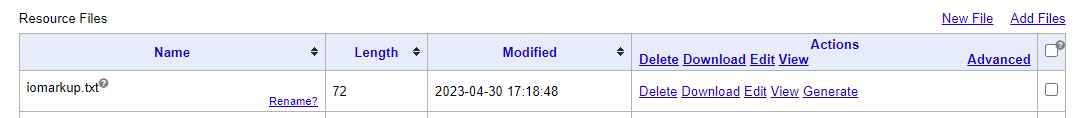
\includegraphics[scale=0.6]{img/files.png}
\end{figure}

На странице генерации пользователь выбирает какие программные компоненты нужно сгенерировать и на каких языках программирования. Страница с выбором показана на рисунке~\ref{generate-screenshot}.

\begin{figure}[!h]
\caption{Выбор параметров генерации}\label{generate-screenshot}
\centering
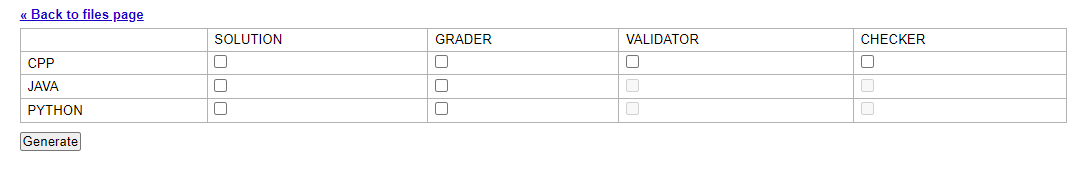
\includegraphics[scale=0.6]{img/generate.png}
\end{figure}

\subsection{Сервис кодогенерации}

В силу особенностей используемой библиотеки, реализующей протокол XML-RPC, реализация конечной точки обработки запроса на генерацию кода представлена реализацией интерфейса \texttt{com.codeforces.interop.iomarkup.InteropRpc} классом \texttt{InteropRpcImpl}. При получении запроса, происходит десериализация тела запроса на генерацию из массива байт, затем обработка запроса по алгоритмам, описанным выше в работе и сериализация ответа с помощью Protobuf в массив байт. При возникновении ошибки обработка прекращается и ответ, содержащий описание ошибки, возвращается немедленно.

\section{Тестирование}

Тестирование предложенного в данной работе решения производилось на нескольких соревнованиях на платформе Codeforces. Для задач соревнований были вручную написаны описания входных и выходных данных и сгенерированны валидатор, чекер и грейдеры. Для каждого сгенерированного компонента на каждом языке проверялось, что сгенерированный код компилируется без ошибок (в случае Python проверялась корректности синтаксиса).

Рассмотрим множество всех возможных файлов. Валидатор для задачи должен выдавать положительный результат (вердикт <<корректный тест>>) на подмножестве этого множества. При этом, сгенерированный валидатор должен выдавать положительный результат для подмножества множества всех возможных файлов, но, для надмножества множества корректных тестов, определяемых <<настоящим>> валидатором. Иными словами, не должно быть такого файла, для которого <<настоящий валидатор>> выдаст вердикт <<корректный тест>>, а сгенерированный~--- <<некорректный тест>>.

Для каждой задачи при тестировании автоматически загружался пакет задачи из <<Polygon>>. Для каждого теста валидатора, для которого валидатор из пакета задачи выдавал вердикт <<корректный тест>> проверялось, что сгенерированный валидатор выдавал такой же вердикт. Для всех наборов входных данных из пакета задачи проверялось, что сгенерированный валидатор выдает вердикт <<корректный тест>> на каждом из них. 

Тестирование происходило в условиях, максимально приближенных к тем, в которых происходит тестирование на платформах <<Codeforces>> и <<Polygon>>. Для этого проект <<Invoker>>, который реализует полный цикл тестирования на вышеупомянутых платформах, был подготовлен для использования в качестве отдельной библиотеки и добавлен в качестве тестовой зависимости в реализацию решения в данной работе.

\chapterconclusion

В этой главе был описан процесс частичной генерации исходного кода валидатора, чекера и грейдеров на основании обработанного описания входных и выходных данных. Описан способ интеграции в систему подготовки задач по спортивному программированию <<Polygon>>. Описан процесс тестирования реализованной системы кодогенерации.

\startconclusionpage

В данной выпускной квалификационной работе была разработана система, частично автоматизирующая процесс построения программных компонентов~--- чекера, валидатора и грейдеров~--- при подготовке задач по спортивному программированию.

Был спроектирован язык описания входных и выходных данных, позволяющий описывать структуру и формат файлов ввода и вывода для задачи. Реализована и описана система частичной генерации исходных кодов валидатора, чекера и грейдеров, включающих в себя реализацию ввода-вывода данных, описание структур, необходимых в задаче, а так же проверку логических условий, заданных автором. Система позволяет частично генерировать исходный код валидатора и чекера на языке программирования C++ с использованием библиотеки \texttt{testlib.h}, а так же генерировать исходный код грейдеров на языках программирования C++, Java и Python.

Реализованная система интегрирована в сервис для подготовки задач по спортивному программированию <<Polygon>>, на работу получен акт о внедрении.

В дальнейшем планируется доработка системы: добавление возможности генерации исходных кодов генераторов и секций <<входные данные>> и <<выходные данные>> в условиях задач.

\printmainbibliography

\appendix

\chapter{Условие задачи <<Копия копии копии>>}\label{statement1772F}

% \begin{problem}{Копия копии копии}{стандартный ввод}{стандартный вывод}{2 секунды}{256 мегабайт}

Все началось с черно-белой картинки, которую можно представить как матрицу $n \times m$ такую, что все ее элементы равны $0$ или $1$. Строки пронумерованы от $1$ до $n$, столбцы пронумерованы от $1$ до $m$.

Над картинкой проделали несколько операций (возможно, ноль), каждая~--- одного из двух типов:
\begin{itemize}[leftmargin=1.75cm]
\item выбрать ячейку такую, что она не находится на границе (строка не $1$ и не $n$, столбец не $1$ и не $m$) и она окружена четырьмя ячейками противоположного цвета (четырьмя нулями, если она единица, и наоборот), и перекрасить ее саму в противоположный цвет;
\item сделать копию текущей картинки.
\end{itemize}

Обратите внимание, что порядок операций мог быть произвольным, они могут не чередоваться.

Вам сообщили результат: все $k$ копий, которые были сделаны. Кроме того, вам сообщили первоначальную картинку. Однако, все эти $k+1$ картинки были перемешаны.

Восстановите последовательность операций. Если существует несколько ответов, то выведите любой из них. Тесты построены из реальной последовательности операций, т.\,е. хотя бы один ответ всегда существует.

%\InputFile

\textbf{Формат входных данных}

В первой строке записаны три целых числа $n, m$ и $k$ ($3 \le n, m \le 30$;~$0 \le k \le 100$)~--- количество строк, количество столбцов и количество сделанных копий, соответственно.

Затем следуют $k+1$ картинок~--- $k$ копий и первоначальная. Их порядок произвольный.

Каждая картинка состоит из $n$ строк, в каждой по $m$ символов, каждый символ~--- это $0$ или $1$. \textbf{Перед каждой картинкой идет пустая строка.}

%\OutputFile

\textbf{Формат выходных данных}

В первой строке выведите одно целое число~--- номер первоначальной картинки. Картинки пронумерованы от $1$ до $k+1$ в порядке, в котором они заданы во входных данных.

Во второй строке выведите одно целое число $q$~--- количество операций.

В каждой из следующих $q$ строк должна быть записана одна операция. Операции должны быть перечислены в том порядке, в котором они применялись. Каждая операция может быть одного из двух типов:
\begin{itemize}[leftmargin=1.75cm]
\item $1$ $x$ $y$~--- перекрасить ячейку $(x, y)$ ($y$-я ячейка в $x$-й строке, она не должна лежать на границу и должна быть окружена четырьмя клетками противоположного от себя цвета);
\item $2$ $i$~--- сделать копию текущей картинки и присвоить ей номер $i$ (картинка под номером $i$ должна совпадать с текущей картинкой).
\end{itemize}

Каждый номер от $1$ до $k+1$ должен встречаться в выводе ровно один раз~--- один из них~--- это номер первоначальной картинки, остальные $k$~--- аргументы операций второго типа.

Если существует несколько ответов, то выведите любой из них. Тесты построены из реальной последовательности операций, т.\,е. хотя бы один ответ всегда существует.

%\Examples
% todo
%\textbf{Примеры}
%
%\begin{table}[!h]
%\centering
%\begin{tabular}{|*{2}{c|}}\hline
%Стандартный ввод & Стандартный вывод \\\hline
%\texttt{3 3 1
%
%010
%111
%010
%
%010
%101
%010}
% & 17 \\\hline
%32 & 34 \\\hline
%48 & 51 \\\hline
%64 & 68 \\\hline
%\end{tabular}
%\end{table}

% \begin{table}[!h]
% \centering
% \begin{tabularx}{\textwidth}{|*{2}{>{\centering\arraybackslash}X|}}\hline
% Стандартный ввод & Стандартный ввод \\\hline
% \begin{minipage}[t]{0.43}16\end{minipage} & 17 \\\hline
% 32 & 34 \\\hline
% 48 & 51 \\\hline
% 64 & 68 \\\hline
% \end{tabularx}
% \end{table}

%\begin{example}
%\exmpfile{example.01}{example.01.a}%
%\exmpfile{example.02}{example.02.a}%
%\exmpfile{example.03}{example.03.a}%
%\end{example}

% \end{problem}

\chapter{Грамматика языка описания}\label{appendix-antlr-grammar}

\begin{lstlisting}[
    caption={Определения токенов в формате ANTLR 4},
    keywordstyle=\color{black},
    commentstyle=\color{black},
    stringstyle=\color{black},
    label={appendix-lexer-src}
]
LINE_COMMENT: '#' .*? '\r'? ('\n' | EOF) -> skip;
COMMENT: '/*' .*? '*/' -> skip;

fragment ESCAPED_CHAR: '\\n';

CHAR: '\'' ((~['\\\r\n]) | ESCAPED_CHAR) '\'';
STRING: '"' ((~["\\\r\n]) | ESCAPED_CHAR)* '"';
TRUE: 'true';
FALSE: 'false';
LOGICAL_AND: '&&';
LOGICAL_OR: '||';
LOGICAL_NOT: '!';
BITWISE_AND: '&';
BITWISE_XOR: '^';
PIPE: '|';
BITWISE_NOT: '~';
EQUALS: '==';
NOT_EQUALS: '!=';
LESS_EQUAL: '<=';
GREATER_EQUAL: '>=';
LESS: '<';
GREATER: '>';
PLUS: '+';
MINUS: '-';
POW: '**';
MULTIPLICATION: '*';
DIVISION: '/';
MODULO: '%';
DOT: '.';
COLON: ':';
QUESTION: '?';
ASSIGN: '=';
COMMA: ',';
SEMICOLON: ';';
LBRACE: '{';
RBRACE: '}';
LBRACKET: '[';
RBRACKET: ']';
LPAR: '(';
RPAR: ')';
SEP: 'sep';
EOLN_MODIFIER: 'eoln';
IF: 'if';
ARRAY: 'array';
OF: 'of';
ELSE: 'else';

fragment U_NUM_LITERAL_MODIFIER: 'u' | 'U';
fragment L_NUM_LITERAL_MODIFIER: 'l' | 'L';
fragment F_NUM_LITERAL_MODIFIER: 'f' | 'F';
fragment EXPONENT: 'e' | 'E';
fragment DIGITS: [0-9][0-9'_]*;

fragment INTEGER_SUFFIX: U_NUM_LITERAL_MODIFIER? L_NUM_LITERAL_MODIFIER?;
fragment FLOAT_SUFFIX: ('.' DIGITS)? (EXPONENT DIGITS)? F_NUM_LITERAL_MODIFIER?;

NUM_VALUE: DIGITS INTEGER_SUFFIX FLOAT_SUFFIX;

NAME: [a-zA-Z_][a-zA-Z0-9_]*;
WS: [ \t\r\n]+ -> skip;
\end{lstlisting}

\begin{lstlisting}[
    caption={Грамматика языка описания в формате ANTLR 4},
    keywordstyle=\color{black},
    commentstyle=\color{black},
    stringstyle=\color{black},
    label={appendix-grammar-src}
]
ioMarkup: (namedStruct)* EOF;
namedStruct: NAME namedStructParameters? struct;
namedStructParameters: LPAR (parameterDeclaration (COMMA parameterDeclaration)*)? RPAR;
parameterDeclaration: NAME COLON namedType;
struct: LBRACE structItem* RBRACE;
structItem: conditionalAlternative | variableDeclaration | ioModifier;
conditionalAlternative: IF LPAR plExpression RPAR struct (ELSE struct)?;
ioModifier: EOLN_MODIFIER SEMICOLON;
variableDeclaration: NAME COLON variableType variableConstraint? SEMICOLON;
variableType: arrayOfUnnamedStruct | (namedType namedTypeParameters? arrayParameters*);
arrayOfUnnamedStruct: ARRAY arrayParameters+ OF struct;
variableConstraint: PIPE plExpression;
namedType: NAME;
namedTypeParameters: LPAR (plExpression (COMMA plExpression)*)? RPAR;
arrayParameters: LBRACKET arrayIterationRange (COMMA SEP ASSIGN sepValue) RBRACKET;
arrayIterationRange: NAME ASSIGN plExpression DOT DOT plExpression;
sepValue: STRING | CHAR;
\end{lstlisting}

\begin{lstlisting}[
    caption={Грамматика языка выражений в формате ANTLR 4},
    keywordstyle=\color{black},
    commentstyle=\color{black},
    stringstyle=\color{black},
    label={appendix-grammar-pl-src}
]
plExpression: plImplLogicalOr (QUESTION plImplLogicalOr COLON plImplLogicalOr)?;

plImplLogicalOr: plImplLogicalAnd (LOGICAL_OR plImplLogicalAnd)*;
plImplLogicalAnd: plImplBitwiseOr (LOGICAL_AND plImplBitwiseOr)*;
plImplBitwiseOr: plImplBitwiseXor (PIPE plImplBitwiseXor)*;
plImplBitwiseXor: plImplBitwiseAnd (BITWISE_XOR plImplBitwiseAnd)*;
plImplBitwiseAnd: plImplEquality (BITWISE_AND plImplEquality)*;
plImplEquality: plImplRelational (plImplEqualityOp plImplRelational)*;
plImplRelational: plImplBitwiseShift (plImplRelationalOp plImplBitwiseShift)?;
plImplBitwiseShift: plImplAdditiveBinary (plImplBitwiseShiftOp plImplAdditiveBinary)?;
plImplAdditiveBinary: plImplMultiplicativeBinary (plImplAdditiveOp plImplMultiplicativeBinary)*;
plImplMultiplicativeBinary: plImplPowBinary (plImplMultiplicativeBinaryOp plImplPowBinary)*;
plImplPowBinary: plImplPrefixUnary (POW plImplPrefixUnary)*;
plImplPrefixUnary: plImplPrefixUnaryOp* plImplHighestPriority;

plImplHighestPriority: ((LPAR plExpression RPAR) | plFunctionCall | plValue | plVarBinding) plSubscript*;

plImplEqualityOp: EQUALS | NOT_EQUALS;
plImplRelationalOp: GREATER | LESS | GREATER_EQUAL | LESS_EQUAL;
plImplAdditiveOp: PLUS | MINUS;
plImplMultiplicativeBinaryOp: MULTIPLICATION | DIVISION | MODULO;
plImplPrefixUnaryOp: LOGICAL_NOT | BITWISE_NOT | MINUS;
plImplBitwiseShiftOp: LESS LESS | GREATER GREATER;

plFunctionCall: NAME LPAR plImplFunctionArgs? RPAR;
plImplFunctionArgs: plExpression (COMMA plExpression)*;

plVarBinding: NAME;

plSubscript: LBRACKET plExpression RBRACKET;

plValue: plNumValue | plBoolValue | plCharValue | plStringValue;
plBoolValue: TRUE | FALSE;
plCharValue: CHAR;
plStringValue: STRING;
plNumValue: NUM_VALUE;
\end{lstlisting}

\chapter{Язык записи выражений}\label{appendix-pl-operators-priority}

\begin{table}[!h]
\caption{Операторы языка выражений в порядке уменьшения приоритета}\label{pl-operators-priority}
\centering
\begin{adjustbox}{angle=90}
\begin{tabular}{|*{4}{c|}}\hline
Приоритет & Нетерминал & Оператор & Описание\\\hline
1  & \texttt{plImplHighestPriority} & \texttt{f(x)} & Вызов функции \\\hline
1  & \texttt{plImplHighestPriority} & \texttt{x[y]} & Взятие по индексу \\\hline
2  & \texttt{plImplPrefixUnary} & \texttt{!x} & Логическое отрицание \\\hline
2  & \texttt{plImplPrefixUnary} & \texttt{\textasciitilde{x}} & Инверсия битов \\\hline
2  & \texttt{plImplPrefixUnary} & \texttt{-x} & Унарный минус \\\hline
3  & \texttt{plImplPowBinary} & \texttt{x ** y} & Возведение в степень \\\hline
4  & \texttt{plImplMultiplicativeBinary} & \texttt{x * y} & Умножение \\\hline
4  & \texttt{plImplMultiplicativeBinary} & \texttt{x / y} & Деление \\\hline
4  & \texttt{plImplMultiplicativeBinary} & \texttt{x \% y} & Остаток от деления \\\hline
5  & \texttt{plImplAdditiveBinary} & \texttt{x + y} & Сложение \\\hline
5  & \texttt{plImplAdditiveBinary} & \texttt{x - y} & Вычитание \\\hline
6  & \texttt{plImplBitwiseShift} & \texttt{x >{>} y} & Побитовый сдвиг вправо \\\hline
6  & \texttt{plImplBitwiseShift} & \texttt{x <{<} y} & Побитовый сдвиг влево \\\hline
7  & \texttt{plImplRelationalOp} & \texttt{>}, \texttt{<}, \texttt{>=}, \texttt{<=} & Сравнение \\\hline
8  & \texttt{plImplEquality} & \texttt{x == y} & Равенство \\\hline
8  & \texttt{plImplEquality} & \texttt{x != y} & Неравенство \\\hline
9  & \texttt{plImplBitwiseAnd} & \texttt{x \& y} & Побитовое <<И>> \\\hline
10  & \texttt{plImplBitwiseXor}  & \texttt{x \textasciicircum~y} & Побитовое исключающее <<ИЛИ>> \\\hline
11  & \texttt{plImplBitwiseOr}  & \texttt{x | y} & Побитовое <<ИЛИ>> \\\hline
12  & \texttt{plImplLogicalAnd}  & \texttt{x \&\& y} & Конъюнкция \\\hline
13  & \texttt{plImplLogicalOr}  & \texttt{x || y} & Дизъюнкция \\\hline
14  & \texttt{plExpression}  & \texttt{x ? y : x} & Тернарный оператор \\\hline
\end{tabular}
\end{adjustbox}
\end{table}

\chapter{Структура запросов и ответов сервиса генерации}\label{appendix-protobuf}

\begin{lstlisting}[
    caption={Структура запросов и ответов сервиса генерации в формате Protobuf},
    keywordstyle=\color{black},
    commentstyle=\color{black},
    stringstyle=\color{black},
    label={appendix-protobuf-src}
]
syntax = "proto2";

enum TargetLanguage {
    CPP = 0;
    JAVA = 1;
    PYTHON = 2;
}
enum TargetComponent {
    SOLUTION = 0;
    GRADER = 1;
    VALIDATOR = 2;
    CHECKER = 3;
}
message TargetFileDescription {
    required TargetComponent target_component = 1;
    required TargetLanguage target_language = 2;
    optional string name = 3;
    optional string previous_content = 4;
}
message ResultFile {
    required TargetComponent component = 1;
    required TargetLanguage language = 2;
    required string name = 3;
    required string content = 4;
    optional string error_message = 5;
}
message GenerateRequest {
    required string io_markup = 1;
    repeated TargetFileDescription target_file_description = 2;
}
message GenerateResponse {
    repeated ResultFile result_file = 1;
    optional string error_message = 2;
}
\end{lstlisting}

\chapter{Шаблоны генерируемого кода}\label{templates}

Листинги в этом приложении содержат код с незначительными сокращениями.

\begin{lstlisting}[caption={Шаблон исходного кода валидатора},label={templates-validator},language=c++]
#include <iostream>
#include <vector>
#include "testlib.h"
namespace iomarkup
{
    int pow(int a, int b)
    {
        if (b == 0) return 1;
        if (b %% 2 == 1) return a * pow(a, b - 1);
        return pow(a * a, b / 2);
    }
    
    long long pow(long long a, long long b)
    {
        if (b == 0) return 1ll;
        if (b %% 2 == 1) return a * pow(a, b - 1ll);
        return pow(a * a, b / 2ll);
    }
}
using std::cin;
using std::cout;
using std::vector;

// Structure declarations
%s

input_t input;

// Functions for input
%s
            
int main(int argc, char *argv[])
{
    registerValidation(argc, argv);
    input = read_input();
    inf.readEoln();
    inf.readEof();
    
    // Write code for semantic input validation here.
    return 0;
}
\end{lstlisting}


\begin{lstlisting}[caption={Шаблон исходного кода чекера},label={templates-checker},language=c++]
#include <iostream>
#include <vector>
#include "testlib.h"
namespace iomarkup
{
    int pow(int a, int b)
    {
        if (b == 0) return 1;
        if (b %% 2 == 1) return a * pow(a, b - 1);
        return pow(a * a, b / 2);
    }
    
    long long pow(long long a, long long b)
    {
        if (b == 0) return 1ll;
        if (b %% 2 == 1) return a * pow(a, b - 1ll);
        return pow(a * a, b / 2ll);
    }
}
using std::cin;
using std::cout;
using std::vector;

// Structure declarations
%s
input_t input;

// Functions for input
%s

typedef output_t AnsType;
AnsType readAns(InStream& stream)
{
    output_t output = read_output(stream);
    // Write code for semantic check answer here.
    // For example, here you should check a certificate.
    // You should return a comparable representation of answer's quality.
    return output;
}
int main(int argc, char *argv[])
{
    registerTestlibCmd(argc, argv);
    input = read_input(inf);
    AnsType pa_answer = readAns(ouf);
    AnsType jury_answer = readAns(ans);
    // Check here that participant have found answer with the same quality as jury.
    
}
\end{lstlisting}


\begin{lstlisting}[caption={Шаблон исходного кода грейдера на языке C++},label={templates-grader-cpp},language=C++]
#include <iostream>
#include <vector>
namespace iomarkup
{
    int pow(int a, int b)
    {
        if (b == 0) return 1;
        if (b %% 2 == 1) return a * pow(a, b - 1);
        return pow(a * a, b / 2);
    }
    
    long long pow(long long a, long long b)
    {
        if (b == 0) return 1ll;
        if (b %% 2 == 1) return a * pow(a, b - 1ll);
        return pow(a * a, b / 2ll);
    }
}
using std::cin;
using std::cout;
using std::vector;

// Structure declarations
%s
input_t input;
// Functions for input
%s
            
// Functions for output
%s

int main(int argc, char *argv[])
{
    input = read_input();
    write_output(solve(input));
    return 0;
}
\end{lstlisting}


\begin{lstlisting}[caption={Шаблон исходного кода грейдера на языке Java},label={templates-grader-java},language=Java]
public abstract class Grader {
    private static class IoMarkup {
        private IoMarkup() {}
        int pow(int a, int b) {
            if (b == 0) return 1;
            if (b % 2 == 1) return a * pow(a, b - 1);
            return pow(a * a, b / 2);
        }
        long pow(long a, long b) {
            if (b == 0) return 1L;
            if (b % 2 == 1) return a * pow(a, b - 1L);
            return pow(a * a, b / 2L);
        }
    }

    // Structure declarations
    %s

    private final java.util.Scanner in;
    private final java.io.PrintStream out;
    private Input input;

    public Solution(java.util.Scanner in, java.io.PrintStream out) {
        this.in = in;
        this.out = out;
    }

    // Input methods
    %s
    
    // Output methods
    %s

    public abstract Output solve(Input input);

    public static void main(java.lang.String[] args) {
        try (java.util.Scanner inputScanner =
                new java.util.Scanner(java.lang.System.in)) {
            Solution solution = new Solution(
                inputScanner, java.lang.System.out);
            solution.input = solution.readInput();
            solution.writeOutput(solution.solve(solution.input));
        }
    }
}
\end{lstlisting}


\begin{lstlisting}[caption={Шаблон исходного кода грейдера на языке Python},label={templates-grader-python},language=Python]
import solution

def iomarkup_div(x, y):
    return x / y if isinstance(x, float) or \
        isinstance(y, float) else x // y

class Scanner:
    def __init__(self, next_line_getter):
        self._next_line_getter = next_line_getter
        self._tokens = []
        self._i = 0
        self._j = None

    def _ensure_token(self):
        if self._i >= len(self._tokens):
            self._tokens.extend(
                self._next_line_getter().strip().split())

    def next(self):
        self._ensure_token()
        next_token = self._tokens[self._i]
        if self._j is not None:
            next_token = next_token[self._j:]
        self._i += 1
        self._j = None
        return next_token

    def next_int(self):
        return int(self.next())

    def next_float(self):
        return float(self.next())

    def next_char(self):
        self._ensure_token()
        next_token = self._tokens[self._i]
        if self._j is not None:
            if self._j >= len(next_token):
                self._i += 1
                self._j = None
                return self.next_char()
            next_token = next_token[self._j]
            self._j += 1
        else:
            self._j = 1
            next_token = next_token[0]
        return next_token

    def next_bool(self):
        return self.next() == "true"

    @staticmethod
    def from_input():
        return Scanner(input)

_scanner = Scanner.from_input()

# Structure declarations
%s

input = None

# Input functions
%s

# Output functions
%s

if __name__ == '__main__':
    input = read_input()
    write_output(solution.solve(input))
\end{lstlisting}

\chapter{Примеры генерируемого кода}

В этом приложении приведены сгенерированные программные компоненты задачи <<Копия копии копии>> из приложения~\ref{statement1772F}. Соответствующее описание входных и выходных данных приведено в разделе~\ref{lang-concepts} в листинге~\ref{iomarkupfullexample}. Здесь будут приведены части кода до вставки в шаблоны из приложения~\ref{templates} с некоторыми незначительными сокращениями.

\begin{lstlisting}[caption={Часть сгенерированного кода валидатора на языке C++},label={gen-val-cpp},language=C++]
input_t read_input();
picture_t read_picture(int n, int m);

input_t read_input()
{
    input_t input;
    input.n = inf.readInt();
    ensuref((3 <= input.n) && (input.n <= 30));
    inf.readSpace();
    input.m = inf.readInt();
    ensuref((3 <= input.m) && (input.m <= 30));
    inf.readSpace();
    input.k = inf.readInt();
    ensuref((0 <= input.k) && (input.k <= 100));
    inf.readEoln();
    inf.readEoln();
    for (int i = 1; i <= (input.k + 1); i++)
    {
        if (i != 1)
        {
            inf.readEoln();
            inf.readEoln();
        }
        picture_t tmp;
        tmp = read_picture(input.n, input.m);
        input.pictures.push_back(tmp);
    }
    return input;
}

picture_t read_picture(int n, int m)
{
    picture_t picture;
    for (int i = 1; i <= n; i++)
    {
        if (i != 1)
        {
            inf.readEoln();
        }
        std::string tmp;
        tmp = inf.readToken();
        picture.s.push_back(tmp);
        ensuref(picture.s[i - 1].size() == m);
    }
    return picture;
}
\end{lstlisting}

\begin{lstlisting}[caption={Часть сгенерированного кода чекера на языке C++},label={gen-checker-cpp},language=C++]
output_t read_output(InStream& stream);
input_t read_input(InStream& stream);
picture_t read_picture(InStream& stream, int n, int m);
ops_t read_ops(InStream& stream);

output_t read_output(InStream& stream)
{
    output_t output;
    output.startPicIndex = stream.readInt();
    output.q = stream.readInt();
    for (int j = 1; j <= output.q; j++)
    {
        ops_t tmp;
        tmp = read_ops(stream);
        output.ops.push_back(tmp);
    }
    return output;
}

input_t read_input(InStream& stream)
{
    input_t input;
    input.n = stream.readInt();
    input.m = stream.readInt();
    input.k = stream.readInt();
    for (int i = 1; i <= (input.k + 1); i++)
    {
        picture_t tmp;
        tmp = read_picture(stream, input.n, input.m);
        input.pictures.push_back(tmp);
    }
    return input;
}

picture_t read_picture(InStream& stream, int n, int m)
{
    picture_t picture;
    for (int i = 1; i <= n; i++)
    {
        std::string tmp;
        tmp = stream.readToken();
        picture.s.push_back(tmp);
    }
    return picture;
}

ops_t read_ops(InStream& stream)
{
    ops_t ops;
    ops.op = stream.readInt();
    if (ops.op == 1)
    {
        ops.x = stream.readInt();
        ops.y = stream.readInt();
    }
    else
    {
        ops.i = stream.readInt();
    }
    return ops;
}
\end{lstlisting}

\begin{lstlisting}[caption={Часть сгенерированного кода грейдера на языке C++},label={gen-grader-cpp},language=C++]
input_t read_input();
picture_t read_picture(int n, int m);

output_t read_output()
{
    output_t output;
    cin >> output.startPicIndex;
    cin >> output.q;
    for (int j = 1; j <= output.q; j++)
    {
        ops_t tmp;
        tmp = read_ops();
        output.ops.push_back(tmp);
    }
    return output;
}

input_t read_input()
{
    input_t input;
    cin >> input.n;
    cin >> input.m;
    cin >> input.k;
    for (int i = 1; i <= (input.k + 1); i++)
    {
        picture_t tmp;
        tmp = read_picture(input.n, input.m);
        input.pictures.push_back(tmp);
    }
    return input;
}

picture_t read_picture(int n, int m)
{
    picture_t picture;
    for (int i = 1; i <= n; i++)
    {
        std::string tmp;
        cin >> tmp;
        picture.s.push_back(tmp);
    }
    return picture;
}

void write_output(output_t const& output);
void write_ops(ops_t const& ops);

void write_output(output_t const& output)
{
    cout << output.startPicIndex;
    cout << endl;
    cout << output.q;
    cout << endl;
    for (int j = 1; j <= output.q; j++)
    {
        write_ops(output.ops[j - 1]);
        cout << endl;
    }
}

void write_ops(ops_t const& ops)
{
    cout << ops.op;
    cout << ' ';
    if (ops.op == 1)
    {
        cout << ops.x;
        cout << ' ';
        cout << ops.y;
    }
    else
    {
        cout << ops.i;
    }
}
\end{lstlisting}


\begin{lstlisting}[caption={Часть сгенерированного кода грейдера на языке Java},label={gen-grader-java},language=Java]
private static class Ops {
    private Integer op;
    private Integer x;
    private Integer y;
    private Integer i;
};
    
private static class Picture {
    private java.util.List<java.lang.String> s =
        new java.util.ArrayList<>();
};
    
private static class Input {
    private Integer n;
    private Integer m;
    private Integer k;
    private java.util.List<Picture> pictures =
        new java.util.ArrayList<>();
};
    
private static class Output {
    private Integer startPicIndex;
    private Integer q;
    private java.util.List<Ops> ops = new java.util.ArrayList<>();
};

private Input readInput(){
    Input input = new Input();
    input.n = in.nextInt();
    input.m = in.nextInt();
    input.k = in.nextInt();
    for (Integer i = 1; i <= input.k + 1; i++) {
        Picture tmp;
        tmp = readPicture(input.n, input.m);
        input.pictures.add(tmp);
    }
    return input;
}

private Picture readPicture(Integer n, Integer m){
    Picture picture = new Picture();
    for (Integer i = 1; i <= n; i++) {
        java.lang.String tmp;
        tmp = in.next();
        picture.s.add(tmp);
    }
    return picture;
}
    
private void writeOutput(Output output) {
    out.print(output.startPicIndex);
    out.println();
    out.print(output.q);
    out.println();
    for (Integer j = 1; j <= output.q; j++) {
        writeOps(output.ops.get(j - 1));
        out.println();
    }
}

private void writeOps(Ops ops){
    out.print(ops.op);
    out.print(' ');
    if (ops.op == 1) {
        out.print(ops.x);
        out.print(' ');
        out.print(ops.y);
    } else {
        out.print(ops.i);
    }
}
\end{lstlisting}

\begin{lstlisting}[caption={Часть сгенерированного кода грейдера на языке Java},label={gen-grader-python},language=Python]
class Ops:
    def __init__(self):
        self.op = None
        self.x = None
        self.y = None
        self.i = None

class Picture:
    def __init__(self):
        self.s = []

class Input:
    def __init__(self):
        self.n = None
        self.m = None
        self.k = None
        self.pictures = []

class Output:
    def __init__(self):
        self.startPicIndex = None
        self.q = None
        self.ops = []

def read_input():
    input = Input()
    input.n = _scanner.next_int()
    input.m = _scanner.next_int()
    input.k = _scanner.next_int()
    for i in range(1, (input.k + 1) + 1):
        tmp = read_picture(input.n, input.m)
        input.pictures.append(tmp)
    return input

def read_picture(n, m):
    picture = Picture()
    for i in range(1, (n) + 1):
        tmp = _scanner.next()
        picture.s.append(tmp)
    return picture

def write_output(output):
    print(output.startPicIndex, end='')
    print()
    print(output.q, end='')
    print()
    for j in range(1, (output.q) + 1):
        write_ops(output.ops[(j) - (1)])
        print()

def write_ops(ops):
    print(ops.op, end='')
    print(end=' ')
    if ops.op == 1:
        print(ops.x, end='')
        print(end=' ')
        print(ops.y, end='')
    else:
        print(ops.i, end='')
\end{lstlisting}

\end{document}
